\chapter{Unimodal Black-box Models}\label{chapter:uni_modality}
\textit{``Prediction is very difficult, especially if it's about the future''}-
Niels Bohr

\section{Chapter Overview} 
An accurate diagnosis and prognosis decision generated by a clinical decision support system~(CDSS)~(e.g., cancer) is specific to patients with particular genomic profiles and molecular traits, which needs to address carefully. For example, in cancer diagnosis, discovery of important biomarkers is becoming an important step to understand molecular mechanisms of carcinogenesis in which omics data and clinical outcomes need to be analyzed before making any clinical decision. In particular, CNVs that found to be associated with the risk toward individual cancers, can be analyzed to reveal genetic predispositions before the cancer actually grows. However, complex nature, high dimensionality, and heterogeneity of CNVs make the overall analysis very challenging. Deep learning~(DL)-based approaches can be used to overcome these challenges. While a convolutional neural network~(CNN), which is good at reducing frequency variations and a long short-term memory~(LSTM), which is good at temporal modeling from genomics data can be applied effectively. Further, a neural ensemble method, which can combine several deep architectures is found to be more effective than structures solely based on CNN or LSTM.

\hspace*{3.5mm} In this chapter, we analyse only CNV data, i.e., single modality and try to find association with cancer, a partial effort to develop a CDSS to answer to research question 1\footnote{\textbf{RQ1}: How the multimodal data can be more effective to provide accurate decision, e.g., how to accurately predict the outcome of a diagnosis decision?}?. We collect genomics data about 8,000 cancer patients covering 14 different cancer types from The Cancer Genome Atlas~(TCGA). We extract CNVs features based on 578 oncogenes and 20,308 non-coding human genes, including genomic deletions and duplication across samples using \texttt{MSeq-CNV} tool. Then we train two powerful deep architectures called \texttt{Conv-LSTM} and \texttt{CAE} networks based on two different but sparse representations of CNVs features and create their snapshots models. While the \texttt{Conv-LSTM} can capture locally and globally important features, \texttt{CAE} can utilize unupervised pretraining to initialize the weights in the subsequent convolutional layers to extract most abstract CNV features. Finally, the model averaging ensemble~(MAE) is applied to combine the predictions from the snapshot models and predict the cancer types. We hypothesize\footnote{\textbf{H2}: A neural ensemble method by combining several deep architectures can be more effective than structures solely based on a single model by reducing the generalization error.} that a neural ensemble method by combining several deep architectures can be more effective than structures solely based on a single model by reducing the generalization error.  


\section{Introduction}
With the high-throughput technologies such as next-generation sequencing~(NGS), cancer-specific genetic profiling is now possible. The entire genome sequencing data using NGS can be used to identify similar genetic mutations and genetic variations associated with different tumors. An accurate identification of cancer based on CNVs can help to reveal the genetic predisposition for cancer before cancer actually occurs, so that vigilant prevention and rigorous monitoring may be practiced by those who are highly predisposed. In \cref{chapter:preli}, we discuss how CNVs are associated with individual cancers. Subsequently, CNVs were used to identify minimum redundancy maximum relevance feature selection~(mRMR) and incremental feature selection~(IFS) methods~\cite{zhang2016classification} such that only one sample could be covered at a time or using microarray-based comparative genomic hybridization~(aCGH) methods. Then, the extracted CNVs data were used to train ML and DL models for cancer identification and type prediction. These approaches, are not capable of simultaneous analysis of multiple samples and recurrent CNVs~\cite{malekpour2018mseq}. Although, aCGH methods are more efficient, current aCGH platforms, which benefit from more than 1 million genomic probes, have a lower detection rate of CNVs. 
In this chapter, we emphasize on CNVs-based cancer diagnoses. First, we use MSeq-CNV~\cite{malekpour2018mseq}\footnote{\url{https://github.com/CNVdetection/MSeq-CNV}} to extract the recurrent CNVs. Since MSeq-CNV uses mixture density for modeling aberrations in depth of coverage and abnormalities in the mate pair insertion sizes, common CNVs across multiple samples can be detected easily. CNVs are usually very high dimensional and dynamic data. We hypothesize that the neural ensemble method can be very effective to analyze such high dimensional data through a hierarchical learning process. We train and evaluate \texttt{Conv-LSTM} and \texttt{CAE} networks separately, which follow the model weighted averaging ensemble of the classifiers, where we combine the predictions of multiple model snapshots from these networks.  %Further, we provide interpretations about the prediction made by the neural network in order to make the cancer diagnosis more effective. 
\iffalse
The contributions of this chapter can be summarized as follows:
\vspace{-2mm} 
\begin{itemize}[noitemsep]
    \item We employed MSeq-CNV tool to extract CNVs from protein-coding genes and oncogenes giving a rich-labelled CNVs dataset. 
    \item We propose an effective way of training two deep architectures, such as \texttt{Conv-LSTM} and \texttt{CAE} networks, to capture locally and globally important features, in which unsupervised pretraining is performed to combat the data sparsity. 
    \item We applied MAE to combine the predictions of multiple snapshots from \texttt{Conv-LSTM} and \texttt{CAE} networks. 
    \item We provide comprehensive evaluations with detailed analyses and comparisons with the state-of-the-art. 
\end{itemize}
\vspace{-1mm} 
\fi 

\hspace*{3.5mm} The rest of the chapter is structured as follows:
\cref{chapter_3:rw} covers some related works concerning cancer diagnosis based on single modality data and summarize their potential limitations. \Cref{chapter_3:mm} chronicles the detail of the data collection and feature engineering before the network construction and training. \Cref{chapter_3:results} demonstrates the experimental results and discusses key findings of the study. \Cref{chapter_3:conclusion} provides some explanations of the importance and relevance of the study reported, highlights the limitations, and discuss some future works before concluding the chapter. 

\section{Related Work}\label{chapter_3:rw}
%\subsection{Cancer typing methods}
Numerous approaches using mixed data types such as genomic data, bioimaging data, and clinical outcomes are used for analyzing genomics data and decision making for the cancer treatment~\cite{min}. For example, RNA-Seq data is used widely to identify rare and common transcripts, isoforms, and non-coding RNAs in cancer. Whereas, SNP indicates small genomic variations in cancer patients and array-based DNA methylation data is used to provide epigenetic changes in the genome that are useful for early genetic changes of cancer, e.g., early-stage detection of ovarian cancer is now possible~\cite{82Tomczak,95Gaul}. Since DL algorithms can work better with such high dimensional data, recent studies focused on using DNN architectures such as autoencoder, RBM, DBN, MLP, CNN, and RNN in cancer genomics, e.g., literature~\cite{17Danaee} used Stacked Denoising Autoencoder to extract features from the RNA-seq data, which are then fed into SVM and shallow ANN to classify malignant or benign tumor of breasts~\cite{18Chen}. 

\hspace*{3.5mm} DeepCNA is another CNN-based approach proposed for cancer type prediction based on CNVs and chromatin 3D structure with CNN~\cite{yuan2018cancer}. It is very efficient in the case where both CNA and 3D chromatin structures supplied, availability of such resources not always possible as genomics-based cancer detection. Besides, histology and radiological images are used for understanding the genetic and epigenetic cause in cancer analysis~\cite{yuan2018cancer,20Rajanna,23Zheng}. In particular, GISTIC, MutSig, and clustering algorithms are used to visualize genomic and transcription alterations in various cancers at advanced level~\cite{wb}. Besides, X-ray and CRT images~\cite{25Cruz} along with proteomic and genomic assays are also used, which shows great success in cancer prediction and prognosis~\cite{28Zhou}. Often these images are used to generate noninvasive, functional, and molecular imaging modality data called multispectral photoacoustic imaging~\cite{20Rajanna} to detect prostate cancer using K-means and SVM~\cite{23Zheng}. 

\hspace*{3.5mm} Besides, histopathology images are used~\cite{19Cruz, xu} to identify the existence of cancer using CNN. Literature~\cite{17Danaee} used stacked denoising autoencoder to extract features from RNA-seq data and then fed into SVM and shallow ANN to classify malignant or benign tumor of breasts~\cite{18Chen}. DeepCNA is another CNN-based approach for cancer type prediction based on CNVs and chromatin 3D structure~\cite{yuan2018cancer}. Apart from these works, restricted methods have been proposed based on CNVs for cancer risk and type predictions~\cite{ding2014application, zhang2016classification, elsadek2018supervised}. Xiaofan D. et al~\cite{ding2014application} used recurrent CNVs from non-tumor blood cell DNAs of non-cancer subjects about hepatocellular carcinoma, gastric cancer, and colorectal cancer patients. They found to reveal the differences between cancer patients and controls concerning CN losses and CN gains. Although their study can make predictions on the cancer predisposition of an unseen test group of mixed DNAs with high confidence, it is limited to only Caucasian cohort and Korean cohorts. 

\begin{table*}[!ht]
    \caption{Different cancer detection methods, data types, and performance }
    \label{table:stateofart}
    \begin{center}
    \scriptsize
    \vspace{-6mm}
    \begin{tabular}{l|l|l|l|l|l}
        \hline
        \textbf{Reference} & \textbf{Approach} & \textbf{Cancer types} & \textbf{\#Sample} & \textbf{Data type} & \textbf{Accuracy} \\\hline
            Karim et al.~\cite{karim2018a2ic} & DBN/LSTM & 14 primary types & 15,699 & TCGA CNVs & 73\% \\\hline % 2018
            Yuan et al.~\cite{yuan2018cancer} & CNN & 25 primary types & 14,703 & CNA \& 3D cromatin & 90\% \\\hline % 2018
            Sanaa et al.~\cite{elsadek2018supervised} & LR & 6 primary types & 3,480  & CNVs & 85\% \\\hline % 2018
        	Cruz et al.~\cite{19Cruz} & CNN & Breast cancer  & 605 & Slide images & 96\%  \\\hline  % 2017
            Danee et al.~\cite{17Danaee} & MLP & Breast cancer & 1210 & RNA-seq & 94\% \\\hline % 2016
            Ning et al.~\cite{zhang2016classification} & Dagging & 6 primary types & 3,480  & CNVs & 75\% \\\hline % 2016
        	Rajana et al.~\cite{20Rajanna} & Deep NN & Prostate cancer & 807 & Histology & 95\%\\\hline
            Chen et al.~\cite{18Chen} & Shallow NN & Colon cancer  & 590 & Gene expression & 84\% \\ \hline % 2015
            Ahmed et al.~\cite{abdel2016breast} & DBN & Breast cancer  & 569 & Wisconsin BRCA & 99\% \\ \hline % 2015
            Zheng et al.~\cite{23Zheng} & K-means/SVMst cancer & Phenotype & 569 & Wisconsin BRCA & 97.38\% \\ \hline % 2014
            Xiaofan et al.~\cite{ding2014application} & Naïve Bayes & Cancer risk & 640 & Human SNP & 93\% \\ \hline % 2014
        \end{tabular}
        \vspace{-6mm}
    \end{center}
\end{table*}

\hspace*{3.5mm} Ning Z. et al.~\cite{zhang2016classification} used CNVs level of 23,082 genes for 2,916 instances from cBioPortal for Cancer Genomics to classify six different types of cancers, i.e., breasts, bladder urothelial, colon, glioblastoma, kidney, and head and neck squamous cell. They construct a dagging-based classifier in which the feature space was reduced into CNVs of 19 genes using minimum redundancy maximum relevance feature selection~(mRMR) and incremental feature selection~(IFS) methods~\cite{zhang2016classification}. Their approach managed to achieve an accuracy of 75\%, which indicates that only a few genes may play essential roles in differentiating cancer types. Sanaa et al.~\cite{elsadek2018supervised} extended their work in which 7 ML classifiers were trained giving random forest algorithm accuracy of 86\%. Other works used omics data to identify various cancer types e.g. literature~\cite{fakoor} used principal component analysis~(PCA) to extract features from high dimensional GE data, which are then fed into sparse and stacked autoencoders to classify acute myeloid leukemia, breast, and ovarian cancer patients. Whereas, literature~\cite{ibrahim} proposed a multilevel feature selection technique based on DBN and unsupervised active learning from miRNA expression data, which outperforms PCA-based methods for hepatocellular and breast carcinoma identification.

\hspace*{3.5mm} For analyzing genomics data and decision making for cancer treatment, different ML and DL algorithms were trained using mixed data types, such as genomic data, bioimaging data, and clinical outcomes, as shown in \cref{table:stateofart}. These approaches are not only proven to be useful at improving cancer prognosis, diagnosis, and treatments, but also revealed the subtypes information of several cancer types~\cite{66Huang}. For example, RNA-seq data are used more widely to identify rare and common transcripts, isoforms, and non-coding RNAs in cancer. Single nucleotide polymorphism~(SNP) data are used to identify segmental variations across multiple cancer genomes, and array-based DNA methylation sequencing is used to provide epigenetic changes in the genome that are useful for early genetic changes of cancer (e.g., early-stage and metabolomic detection of ovarian cancer is now possible~\cite{82Tomczak,95Gaul}). 

\hspace*{3.5mm} Unlike conventional cancer typing methods that work on analyzing morphological appearances, gene expression levels of the tumor are used to differentiate tumors that have similar histopathological appearances giving more accurate tumor typing results for the colorectal cancer diagnosis~\cite{paroder2006na+}. Different types of somatic mutations data such as point mutation, single nucleotide variation~(SNV), small insertion and deletion~(INDEL), copy number aberration~(CNA), translocation, and CNVs are also used. Literature~\cite{yuan2018cancer} has observed that these types of genomics data are not only associated with complex diseases but also with contribute to the growth of different types of cancers. In particular, literature~\cite{67Calcagno} studied CN changes by comparing healthy and cancer-affected patients, which showed that amplification and deletion of certain genes are more common in certain cancer patients than healthy people. It has been identified that CNVs are associated with the risk of pancreatic cancer~\cite{66Huang}. 

\hspace*{3.5mm} Imaging data such as histology and radiological images are used for understanding genetic and epigenetic causes in cancer analyses~\cite{yuan2018cancer,20Rajanna,23Zheng}. In particular, GISTIC, MutSig, and clustering algorithms are used to visualize genomic and transcription alterations in various cancers at an advanced level~\cite{wb}. X-ray and CRT images~\cite{25Cruz}, along with proteomic and genomic assays, are also used, which show great success in cancer prediction and prognosis~\cite{28Zhou}. These types of images are used to generate noninvasive, functional, and molecular imaging modality data called multispectral photoacoustic imaging~\cite{20Rajanna} in order to detect prostate cancer using K-means and SVM~\cite{23Zheng}. 

\hspace*{3.5mm} CNVs analysis based on different statistical methods are also used to identify significant CN associated with different types of cancers. For example, Fisher's exact~(FE) test is applied on patient and control groups to identify copy numbers for hereditary breast and ovarian cancer~\cite{58Kuusisto}. Although FE is mainly used for CNV analysis~\cite{fish}, ML-based approaches are trending to improve the accuracy of cancer susceptibility, recurrence, and survival prediction~\cite{16Kourou}. The main challenges are, however, accurate extraction of CNVs and dealing with dimensionality. ML algorithms such as Bayesian networks, SVM, and decision trees are applied effectively to extract the most significant CNVs features fro high dimensional data. In comparison with ML-based approaches, recent DL techniques have shown more accurate and promising results for cancer identification in some studies. In particular, CNN is widely applied~\cite{19Cruz} on whole slide images in order to detect cancer regions with a very high degree of precision, which is mainly because CNN can extract deep features from different cohorts simultaneously. 

\hspace*{3.5mm} Literature~\cite{17Danaee} used a stacked denoising autoencoder to extract features from the RNA-seq data, which are then feed into SVM and shallow ANN to classify malignant or benign tumor of breasts~\cite{18Chen}. DeepCNA is another CNN-based approach proposed for cancer type prediction based on CNVs and chromatin 3D structure with CNN~\cite{yuan2018cancer}. Although DeepCNA is very efficient in cases where both CNA and 3D chromatin structures are supplied, the availability of such resources is not always possible, like in genomics-based cancer detection. Therefore, many researchers try to extract genomics data to be consumed by the DNN architectures. Apart from these works, restricted approaches have been proposed based on CNVs for cancer risk and type predictions~\cite{ding2014application, zhang2016classification, elsadek2018supervised}. Xiaofan D. et al.~\cite{ding2014application} used recurrent CNVs from non-tumor blood cell DNAs of non-cancer subjects about hepatocellular carcinoma, gastric cancer, and colorectal cancer patients. They revealed the differences between cancer patients and controls with respect to CN losses and CN gains. Although their study can make predictions on the cancer predisposition of an unseen test group of mixed DNAs with high confidence, it was limited to only Caucasian and Korean cohorts. 

\hspace*{3.5mm} Ning Z. et al.~\cite{zhang2016classification} used CNVs at a level of 23,082 genes for 2,916 instances from cBioPortal for Cancer Genomics to classify 6 different types of cancers, i.e., breasts, bladder urothelial, colon, glioblastoma, kidney, and head-and-neck squamous cell. They construct a dagging-based classifier in which the feature space was reduced into CNVs of 19 genes using mRMR and IFS methods. They managed to achieve an accuracy of 75\%, indicating that only a few genes may play important roles in differentiating cancer types. Sanaa et al.~\cite{elsadek2018supervised} used the same dataset and train 7 different classifiers in which random forest shows 86\% accuracy. %The data used the CNV in variant types of cancers were downloaded from the
In a previous approach~\cite{karim2018a2ic}, we considered CN segmentation as an important feature because it represents number of CNVs at a DNA location. Higher the segmentation mean, the higher the CN would be in that region. Followed by the calculation of the length of a CN and its value based on the difference between the start and end positions of a CNV to extract CNV features. We represented CN loss with negative segmentation means and amplifications of CN with positive segmentation means. CN with segmentation values between a certain range were considered as noise and discarded from rest of the calculation. However, a manual approach for CNV extraction like this often fails to extract non-trivial, high-quality recurrent CNV features in the case of simultaneous analysis of multiple samples~\cite{malekpour2018mseq}. Consequently, we employed MSeq-CNV for more efficient extraction of CNVs. 

\hspace*{3.5mm} %\subsection{Related works on multimodality}
Literature~\cite{liang} proposed to cluster ovarian and breast cancer patients based on multiplatform genomics~(e.g. GE, DNA methylation, and miRNA expression) and clinical data. To deal with such multiplatform data, MAE is used in which latent features are extracted before clustering with the K-means. Ngiam et al.~\cite{NgiamKKNLN11} proposed a multimodal architecture to handle multimodality of audio and video features based on three methods: multimodal fusion, cross-modality learning, and shared representation learning.
While each method uses multimodalities on the feature learning steps, multimodal fusion uses multimodalities in supervised learning and testing. Cross-modality learning used one type of data for both supervised learning and validating, while shared representation learning used one kind of data for supervised learning and testing. The original idea behind the cross-modality learning is to handle multimedia objects where not all data have all modalities. Liang et al.~\cite{liang} adopts a similar architecture for clustering multimodal cancer genomics GE, DNA methylation, and clinical data.

\section{Methods}\label{chapter_3:mm}
In this section, we discuss in detail the data collection, preprocessing, and feature engineering. % in detail. %, followed by the preparation of training, validation, and test sets. 

\subsection{Problem statement}
A CNV sample $x$ consists of a set of $m$ attribute-value pairs $\left(a_{i}, v_{i}\right)$, where $a_i$ is a feature and $v_i$ is its value from $a_{i}$, where both $a_{i}$ and $v_i \in \mathbb{R}^{D}$. %From given $n$ CNV samples $X$ = ${\{x_1,x_2, ..., x_n}\}$ in dataset $D$, where $x \in \mathbb{R}^{D}$. 
Let $X_{1}, X_{2}, \ldots, X_{m}$ be the CNV samples~(independent $m$-dimensional CNV samples~(i.e., $m$ is number of genes)) for the respective genes $G_{1}, G_{2}, \ldots, G_{m}$ respectively, where $X_{i} \in \mathbb{R}^{D}$ $\operatorname{dom}\left(X_{i}\right)$ which is the range of copy numbers for gene $G_{i}$. Let $C$ be the random variable for the class labels, and $\operatorname{dom}(C)=\{1, \ldots, K\},$ where $K$ denotes the total number of classes. If $t=\left\{t . X_{1}, t . X_{2}, \ldots, t . X_{m}\right\}$ denotes a size $m$ tuple of copy numbers for $m$ genes, $T=$ $\left\{\left(t_{1}, c_{1}\right),\left(t_{2}, c_{2}\right), \ldots,\left(t_{n}, c_{n}\right)\right\}$ denotes a training set of $n$ tuples, where $i=\{1,2, \ldots, n\}, c_{i} \in \operatorname{dom}(C)$ is the class label of tuple $t_{i} 
%Let the test set be $S=\left\{t_{1}, t_{2}, \ldots, t_{l}\right\}$ where $l$ is the size of the test set A classifier is a function Class with two arguments, $T$ and $s,$ where $T$ denotes the training samples and $s$ is a testing sample. Function Class returns a class prediction for sample $s .$ The classification accuracy is defined as the number of correct predictions made by the classifier on a set of testing tuples.
%Given a training set $T=\left\{\left(t_{1}, c_{1}\right),\left(t_{2}, c_{2}\right), \ldots,\left(t_{n}, c_{n}\right)\right\},$ where 
%$t_{i}$ are independent $m$-dimensional GE values~(i.e., $m$ is number of genes), 
=\left(t_{i} \cdot X_{1}, t_{i} \cdot X_{2}, \ldots, t_{i} \cdot X_{m}\right), m \gg n$ and $c_{i} \in \operatorname{dom}(\mathrm{C})$ is the class label of the $i^{th}$  tuple. 
First, we extract important features based on oncogenes and non-coding human genes. 
Then we consider classifying an individual $x$ into a specific group or cancer type, where a predictor~(e.g., a classifier) is a function $F: {X}^{(m)} \rightarrow {Y}$, which maps the data instance from a feature space ${X}^{(m)}$ with $m$ input features to a labels $y$ in a target space ${Y}$, where $F(x)=y$ denotes the decision $y$, predicted by $F$. We also assume that $F$ is a `black-box' predictor, whose internal functioning is either unknown~(or partially known) or known but not interpretable by a human. 
 
%In \cref{chapter:uni_modality}, we developed a `black-box' predictor $f$ whose internal functioning is either unknown~(or partially known) to the observer or they are known but not interpretable by a human. In this chapter, instead we denote $\widetilde{f}$- an interpretable predictor, whose internal processing yielding a decision $\widetilde{f}(x)=y$ can be given a symbolic interpretation understandable by a human. %Examples of such predictors include rule-based classifiers, decision trees, decision sets, and rational functions. 

%the classifier $f$ maps an input $x$ to an output $f(x) \in y, f: \mathbb{R}^{d} \mapsto y$.

\subsection{Datasets}
\label{data}
Copy numbers and gene coordinates of different cancer types from TCGA are used in our study, which are hybridized by genome sequencing technology called {affymetrix SNP 6.0}, which allows us to examine the largest number of cases along with the highest probe density~\cite{31Park}. Tumor tissue and healthy tissue samples are collected from each cancer patient, which are curated from the blood, bone marrow, Buccal cell, EBV immortalized, and solid tissues. For consistency across samples, all data were downloaded from the same platform but with different project ID and gender. However, blood-derived healthy samples of only 14 cancer types were downloaded having at least 400 samples, as shown in~\cref{table:alldatadetails}. 

\begin{table} [!ht]
    \small
    \caption{Number of CNV samples across 14 different tumor types used in this chapter}
    \vspace{-2mm}
    \label{table:alldatadetails}
    \centering
    \begin{tabular}{l|l|l|l}
        \hline
        \rowcolor{Gray}
         \textbf{Cohort} & \textbf{\#Tumor sample} & \textbf{\#Healthy sample} & \textbf{Carcinoma type} \\\hline
        COAD & 502 & 468 & Colon cdenocarcinoma \\\hline
        GBM  & 609 & 527 & Glioblastoma multiforme \\\hline
        KIRC & 586 & 530 & Kidney renal clear cell carcinoma  \\\hline
        LGG  & 514 & 487 & Brain lower grade glioma \\\hline
        LUAD & 554 & 591 & Lung adenocarcinoma \\\hline
        LUSC & 524 & 535 & Lung squamous cell carcinoma \\\hline
        OV   & 572 & 546 & Ovarian serous cystadenocarcinoma \\\hline
        UCEC & 548 & 545 & Uterine corpus endometrial carcinoma \\\hline
        BRCA & 1103 & 1103 & Breast invasive carcinoma  \\\hline 
        HNSC & 519 & 562 & Head \& neck squamous cell carcinoma \\\hline 
        THCA & 505 & 513 & Thyroid carcinoma \\\hline 
        PRAD & 501 & 536 & Prostate adenocarcinoma \\\hline 
        STAD & 442 & 464 & Stomach adenocarcinoma \\\hline 
        BLCA & 416 & 397 & Bladder urothelial carcinoma \\\hline 
    \end{tabular}
    \vspace{-2mm}
\end{table}

\iffalse
\begin{table} [h]
\centering
    \scriptsize
    \caption{number of CNV samples across 14 different tumor types}
    \label{table:alldatadetails}
    \vspace{-2mm}
    \begin{tabular}{l|l|l|l}
        \hline
        \rowcolor{Gray}
         \textbf{Cohort} & \textbf{DNA methylation} & \textbf{Copy numbers} & \textbf{Mutations} & \textbf{miRNA} & \textbf{Gene expression} & \textbf{Carcinoma type} \\\hline
            LUSC & 358 & 345 & 178 & 332 & 227 & Lung squamous cell carcinoma \\\hline
            READ & 162 & 164 & 69 & 143 & 71 & Rectum adeno-carcinoma \\%
            GBM  & 405 & 578 & 290 & 501 & 495 & Glioblastoma multiforme \\\hline
            LAML & 194 & 198 & 197 & 187 & 179 & Acute myeloid leukemia	\\%
            HNSC & 310 & 310 & 277 & 309 & 303 & Head \& neck squamous cell carcinoma \\\hline 
            BLCA & 126 & 126 & 99 & 121 & 96 & Bladder urothelial carcinoma \\\hline 
            KIRC & 457 & 457 & 417 & 442 & 431 & Kidney renal clear cell carcinoma  \\\hline
            UCEC & 512 & 511 & 248 & 497 & 333 & Uterine corpus endometrial carcinoma \\\hline
            LUAD & 431 & 357 & 229 & 365 & 355 & Lung adenocarcinoma \\\hline
            OV   & 592 & 577 & 316 & 454 & 581 & Ovarian serous cystadenocarcinoma \\\hline
            BRCA & 888 & 887 & 772 & 870 & 817 & Breast invasive carcinoma  \\\hline
            COAD & 420 & 422 & 155 & 407 & 192 & Colon cdenocarcinoma \\\hline
            %LGG  & 514 & 487 & Brain lower grade glioma \\\hline
            %THCA & 505 & 513 & Thyroid carcinoma \\\hline 
            %PRAD & 501 & 536 & Prostate adenocarcinoma \\\hline 
            %STAD & 442 & 464 & Stomach adenocarcinoma \\\hline 
    \end{tabular}
\end{table}

\fi 

\hspace*{3.5mm} We consider gender an important feature for cancer subtype classification, since tumors such as {BRCA} and {OV} are not common in males, whereas {PRAD} is only common in males. TCGA do not specify if a sample is curated from healthy tissue or tumor tissue, so we downloaded CNV files in separate groups. Each cancer sample is then grouped as primary and blood-derived samples during filtering before dividing them into male and female groups. We also used gene locations in combination with the copy number data, which are available in all patients for each tumor under each TCGA project. Gene coordinates were collected from cytobands using the ensemble library of \texttt{biomaRt} package\footnote{\url{https://www.ensembl.org/biomart}}. Additionally, oncogenes information were downloaded\footnote{TCGA has listed 568 oncogenes till September 2017} from the TCGA portal. 
%An example of a raw sample of GBM tumor is given in \cref{cnv:gbmCNV2}. 
%Each row in the table represents copy number changes at a specific DNA segment. For example, there is a copy number gain in the first row, which is from location 61,735 to 28,43676 in chromosome 1. However, only 557 probes being used to identify this segment change, which is quantified to 0.0548. Negative segment change represents the deletion from that region. 

\hspace*{3.5mm} Initial prepossessing were required to remove noise, empty, or string values from both CNV and gene data. For each cancer type, samples were downloaded into four different groups: healthy samples from male, healthy samples from female, tumor samples from male, and tumor samples from female. Then we preprocessed CNV data for 15,699 separate samples. Then, all the cancer samples and healthy tissue samples were combined. We found that the distribution of copy numbers across tumor samples are very different. For example, BRCA has almost double the samples of most other tumors. Whereas, {STAD} and {BLCA} have fewer samples compared to other tumor samples except for those having samples between 500-600. While, more than 400 THCA samples have 50 to 100 CNVs per sample, and around 50 OV tumor samples have less than 200 CNVs per sample. 

\iffalse
\begin{table} [!ht]
    \vspace{-3mm} 
    \caption{Example of a COAD CNV sample after preprocessing}
    \label{sample:afterpreprocessing}
    \begin{center}
    \small
    \begin{tabular}{l|l|l|l|l|l|l|l}
    \hline
    \rowcolor{Gray}
    \textbf{Chr} & \textbf{Start} & \textbf{End} & \textbf{Length} & \textbf{Segment\_Mean} & \textbf{Gain/Loss} & \textbf{Gender} & \textbf{Type} \\\hline
        1 & 1710664 & 1741164 & 30500 & -1.2237 & 0 & 0 & 1 \\\hline
    	1 &	16577231 &	16637050 &	59819  & 0.4852 &	1 &	0 &	1  \\\hline
    	1 &	16684955 &	16721910 &	36955  & 0.7576 &	1 &	0 &	1  \\\hline
        1 &	16721984 &	16855942 &	133958   & -0.5558 &	0 &	0 &	1  \\\hline 
    \end{tabular}
    \end{center}
    \vspace{-3mm}
\end{table}
\fi 

\hspace*{3.5mm} Although, most tumor samples have copy numbers between 50-400, there are a few samples having more than 1,500, giving on average 226.80 copy numbers per sample. On average, 106.92 copy numbers exist per healthy sample, which is less than half of tumor samples. Usually, healthy human cells have very different copy numbers in terms of location, length, and number and vary in humans. This makes the CNVs of the human genome an utterly complex and dynamic structure. For a cancer-affected patient, this structure becomes even more complex and dynamic as the tumor grows. In general, healthy human cells have completely different copy numbers in terms of location, length, and number from another human. 

\hspace*{3.5mm} We solve this dynamic dimension problem by using gene locations of the human genome since DL models expect fixed dimension inputs only. We selected a fixed number of genes and extracted the copy numbers that overlapped with the gene locations, removing them from the protein non-coding gene because arguably more than 80\% of human genes do not encode any protein. Thus, copy numbers from these regions have little-to-no effect on tumor growth. %By using gene locations, we safely removed copy numbers that fall within non-coding regions and kept those copy numbers that only affect genes.
%In addition, since not all genes are available in every human body and vary from person to person, genes are also variable in the human genome. 
We prepared two different datasets of CNVs based on oncogenes and protein-coding genes that are used to train the Conv-LSTM and CAE networks to get the ensemble from. Additionally, some preprocessed data\footnote{Based on a Master thesis I co-supervised with Dr. Oya Beyan: "Using Deep Neural Networks and Copy Number Variations for Cancer Detection", by Md. Ashiqur Rahman, Software Systems Engineering, RWTH Aachen University, 2018.} were reused. %Data co %\Cref{fig:pipeline} shows the overall processing pipeline of our proposed approach.

\subsection{Feature selection: protein-coding genes}
We used the CNVs of 20,308 protein non-coding genes. Since not all of these genes are responsible for tumor growth, features from irrelevant genes make the CNV data unnecessarily complex. Neural networks then fail to converge the training, resulting in poor performance. Although using protein-encoding genes makes the dimension fixed, 95\% of the features will be empty across the samples (e.g., a sample with 500 CNVs has 19,808 empty features making empty features for 19,808 cases). Using gene locations adds two additional complexities evolved: the curse of dimensionality and sparsity. 

\hspace*{3.5mm} To solve these problems, we perform CNV analysis in combination with 568 oncogenes responsible for the majority of cancer types. While oncogenes are found to be related to tumor growth, it is not confirmed which other genes also responsible for its growth. In such a setting, consecutive genes with non-zero values represent copy number length, and negative or positive segmentation values represent loss and gain, respectively. We hypothesize that DNN will be able to identify those hidden non-linear features. 

\subsection{Feature selection: oncogenes}
There are structural variations in DNA where protein-encoding genes are not present, and these genes have no effect on tumor growth. One way to remove such unnecessary segments is by keeping only those copy numbers that fall within gene regions and discarding the rest using oncogenes, because oncogenes not only control the cell division but are also responsible for gene expression changes due to external or natural causes and could lead to the development of tumor at some point. Thus, by considering only 568 oncogenes, we prepared another CNV representation instead of taking the whole 20,308 genes. 

\hspace*{3.5mm} As stated earlier, the manual CNV feature extraction is not efficient, and the recurrent CNVs from multiple samples are often ignored, we used the MSeq-CNV tool, which is an efficient CNV extraction method. In order to model the number of mate pairs with aberration in the insertion size and Poisson distribution for emitting the read counts, MSeq-CNV applies the binomial distribution-based mixture density on each genomic position. This applies a mixture density for modeling aberrations in depth of coverage and abnormalities in the mate pair insertion sizes. After applying MSeq-CNV, genome-wide copy gain and loss regions are saved in a matrix form, where each row represents a different CNV call with its sample number, start position, end position, and copy number estimation.
 
 \iffalse
\begin{figure}[ht!]
    \centering
    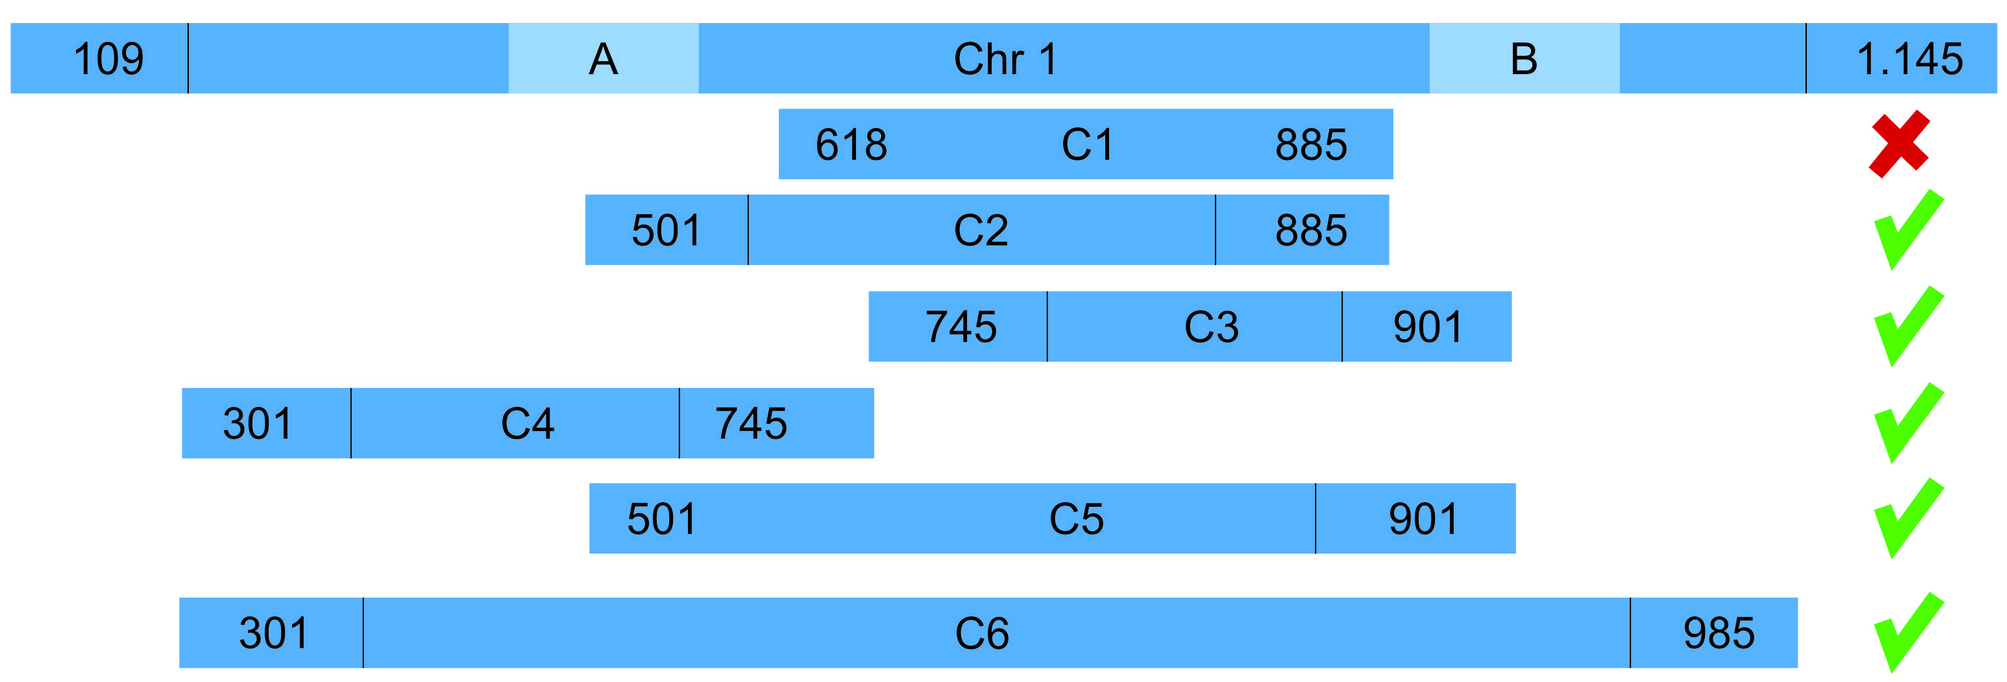
\includegraphics[width=0.90\textwidth,height=55mm]{images/fe.png}
    \caption{CNV selection process using MSeq-CNV}
    \label{fig:cnv_overlap}
\end{figure}
\fi 

%An example of the CNV selection process is shown in \cref{fig:cnv_overlap}. It shows a reference segment of chromosome 1 at the top that extends from DNA location 109 to 1,145 with two genes, A and B, within this segmental region. Below this reference, there are six candidate copy numbers~(C1-C6) at this location. C1 is a candidate copy number that extends between genes A and B, but C1 does not overlap with any one of them, which is why we remove it from the calculation. Candidates C2 and C3 are copy numbers, too, which slightly overlap with A and B, respectively. We still consider them as valid copy numbers because gene positions are not always fixed. C4 and C5 both fully overlap with genes A and B, hence, they are also valid copy numbers. C6 is not only a big segmental copy number, but it also overlaps with both genes. However, since we consider only the part of genes that overlap, we discard rest of the regions from the calculation. This is based on the hypothesis that even if a candidate copy number overlaps with a gene just by one base pair, we still consider it as a valid copy number~\cite{CNV2}. 

\begin{table} [!ht]
    \caption{Example of training data prepared based CNVs representation of oncogenes}
    \label{cnv:changed232d}
    \vspace{-6mm}
    \begin{center}
        \scriptsize
        \begin{tabular}{l|l|l| l|l|l|l|l|l|l}
            \hline
            \rowcolor{Gray}
            \textbf{Type} & \textbf{Gender} & Age & Race & \textbf{PRDM16} & \textbf{RPL22} & \textbf{CAMTA1} & \textbf{MTOR} & .. & \textbf{MTCP1} \\\hline    
            1 & 1 & 45 & American & -0.3195 & -0.2154 & 0 & 0.4767  & .. & 0.652 \\\hline
            2 & 0 & 55 & Indian & 0.230 & -0.552 & 1.715 & -0.92  & .. & -1.0 \\\hline
            3 & 1 & 65 & Nigerian & -1.240 & 0.975 & 0.350 & 0.642  & .. & 0.985 \\\hline
        \end{tabular}
        \vspace{-6mm}
    \end{center}
\end{table}

\hspace*{3.5mm} Each gene has a starting and ending position in DNA, which is similar for copy numbers having starting and ending positions. For each gene, MSeq-CNV checks if a sample has any CNV region overlaps with that gene. Then it assigns the segment value for that gene, otherwise 0 is assigned. This means that a tumor sample has different copy number variation than a reference, which is measured by the segment value. If the value is positive, copy number in that gene is considered to be more increased than the reference. A negative value, however, signifies that the gene was deleted from that DNA location. A sample of the final training data is shown in table \ref{cnv:changed232d}. The first row shows a male patient's GBM tumor sample, where gene PRDM16 and RPL22 have copy number losses with segmentation values of 0.3195 and 0.2154, respectively. Whereas, gene CAMTA1 has no copy number variation, and so on. %Eventually, dimension of the training set reduced from 20,308 to 568 (+ the label column). 

\subsection{Network construction and training}
\label{nc}
We construct and train the Conv-LSTM and CAE networks using two different CNVs representations (i.e., oncogenes and protein-coding genes) in which multiple snapshot models are created. Then, we evaluate each network independently, which is followed by the MEA by combining the snapshot models of both networks. Inspired by literature~\cite{lyu2018deep}, each protein-coding, gene-based CNV was reshaped from a 20,308 x 1 array into a 144 x 144 image, to apply the convolutional~(conv) operations,. Whereas each oncogenes-based CNV sample was reshaped from a 568 x 1 array into 24 x 24 by adding zero padding around the edges. Then, all the images are normalized to [0,255] without losing any information. 

\subsubsection{Construction of Conv-LSTM network }
We construct and train the \texttt{Conv-LSTM} network by combining both CNN and LSTM layers as shown in \cref{fig:conv_lstm}. While the CNN model uses conv filters to capture local relationship values, an LSTM network can carry overall relationship of a whole CNV sequence more efficiently. This turns \texttt{Conv-LSTM} into a powerful architecture to capture long-term dependencies between features extracted by CNN~\cite{karim2019drug}. To capture both the local and global relationships, all the input $\mathcal{X}_{1},\mathcal{X}_{2},...,\mathcal{X}_{t}$ cells in \texttt{Conv-LSTM} output $\mathcal{C}_{1},\mathcal{C}_{2},...,\mathcal{C}_{t}$, hidden states $\mathcal{H}_{1},\mathcal{H}_{2},....,\mathcal{H}_{t}$, and gates $i_t$,$f_t$,$o_t$ of the network as 3D tensors whose last two dimensions are spatial dimensions. %To get a better picture of the inputs and states, we may imagine them as vectors standing on a spatial grid. 
\texttt{Conv-LSTM} determines the future state of a certain cell in the input hyperspace by the inputs and past states of its local neighbors, which is achieved by using a convolution operator in the state-to-state and input-to-state transitions, which can be represented as follows~\cite{Conv_LSTM1,karimACCA2019}:

\vspace{-4mm}
\begin{align}
    \begin{array}{c}
            {i_{t}=\sigma\left(W_{x i} * \mathcal{X}_{t}+W_{h i} * \mathcal{H}_{t-1}+W_{c i} \circ \mathcal{C}_{t-1}+b_{i}\right)} \\
            {f_{t}=\sigma\left(W_{x f} * \mathcal{X}_{t}+W_{h f} * \mathcal{H}_{t-1}+W_{c f} \circ \mathcal{C}_{t-1}+b_{f}\right)} \\
            {\mathcal{C}_{t}=f_{t} \circ \mathcal{C}_{t-1}+i_{t} \circ \tanh \left(W_{x c} * \mathcal{X}_{t}+W_{c o} * \mathcal{C}_{t}+b_{o}\right)} \\
            {\qquad \mathcal{H}_{t}=o_{t} \circ \tanh \left(\mathcal{C}_{t}\right)}
    \end{array}
\end{align}
\vspace{-4mm}

\hspace*{3.5mm} In the above equation,~`*'~denotes the conv operator and `o' is the entrywise multiplication of two matrices of same dimensions. The second LSTM layer emits an output `H', which is then reshaped into a feature sequence and feeds into fully connected layers to predict the cancer types at the next step and as an input at the next time step. Intuitively, an LSTM layer treats an input feature space as timesteps and outputs arbitrary hidden units per timestep. On the other hand, once the input feature space is passed to the conv layer, we pad the input such that the output has the same length as the original input. 

\begin{figure*}
	\centering
	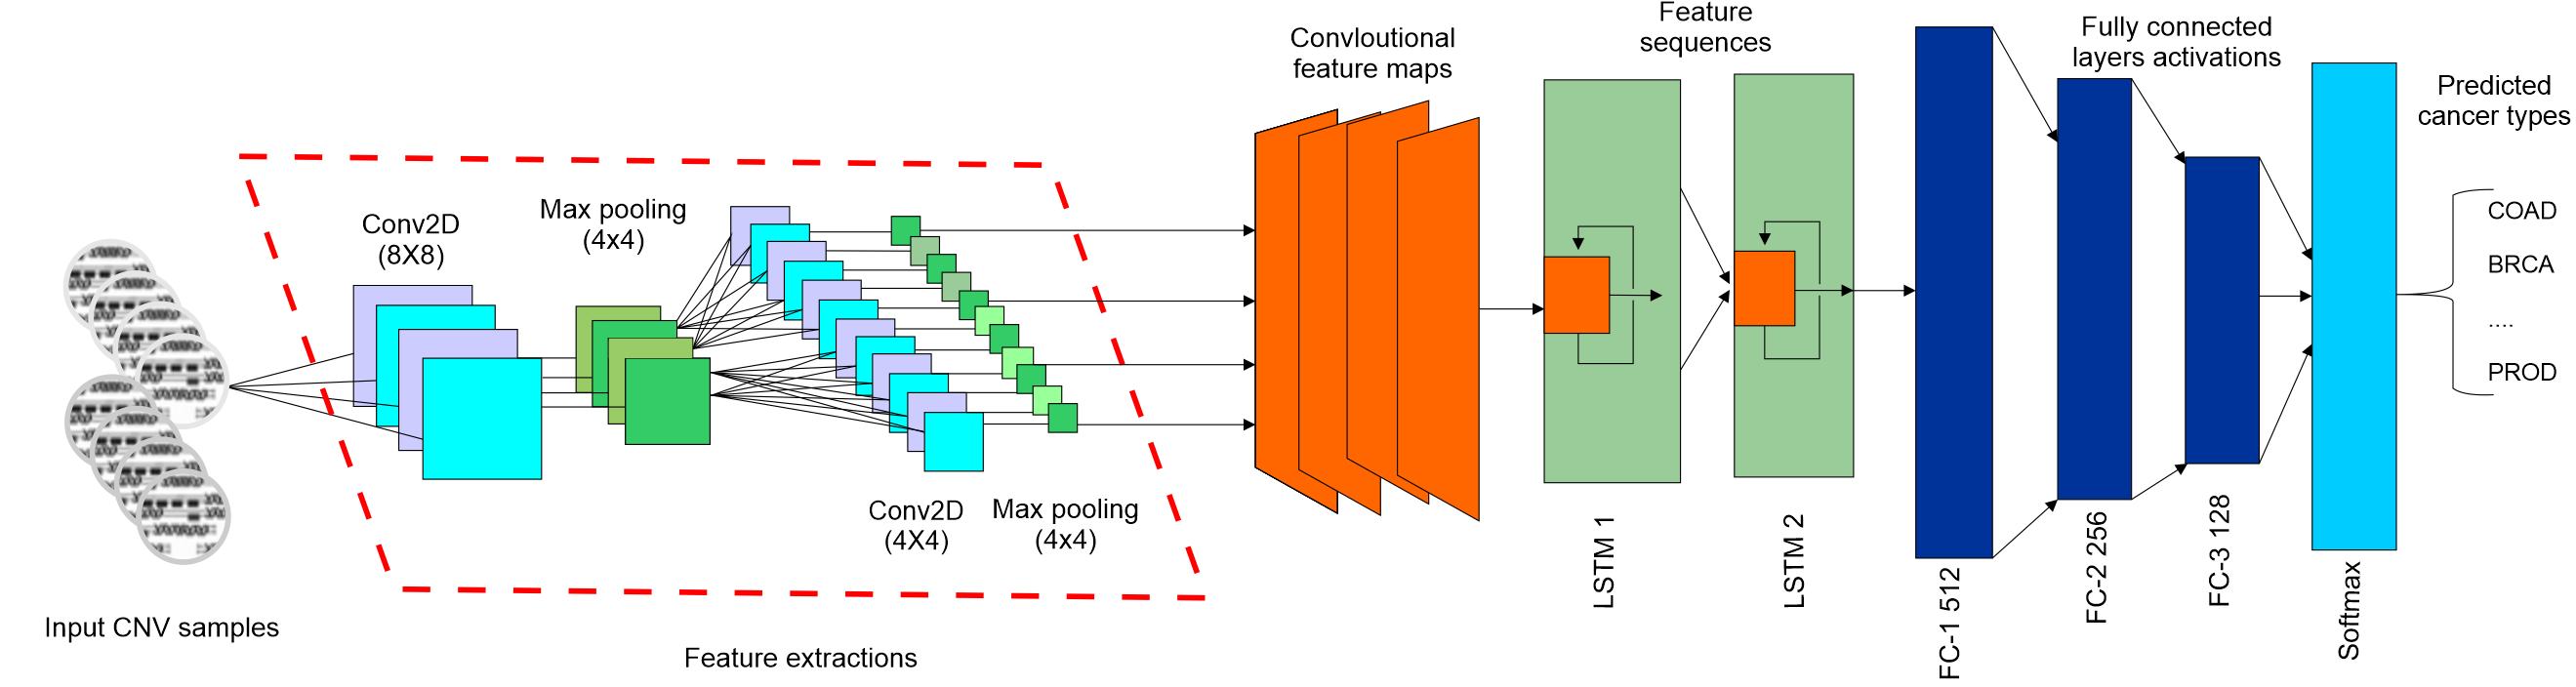
\includegraphics[width=0.80\textwidth,height=40mm]{images/conv_lstm.png}	 
	\caption{Schematic representation of the \texttt{Conv-LSTM} network starts from taking input CNV samples and passing to CNN layers before getting a sequence vector representation from the LSTM layers to pass to dense, dropout, and softmax layers~\cite{karimACCA2019}}	
	\label{fig:conv_lstm}
	\vspace{-2mm}
\end{figure*}

\hspace*{3.5mm} Output of each conv layer is then passed to the dropout layer to regularize learning to avoid overfitting~\cite{vardropout}. This involves the input feature space into lower dimensional representation, which is then further down-sampled by two different max pooling layers and a max pooling layer~(MPL) by setting the pool size. Where the output of an MPL can be considered as an `extracted feature' from each CNV samples. Since each MPL follows to `flatten' the output space by taking the highest value in each timestep dimension, this helps produce a sequence vector, e.g., feature sequence from the last LSTM layer, which will hopefully force the CNV of specific genes that are highly indicative of being responsible for specific cancer type. Then this vector is fed into the neural network after passing through another dropout layer and the softmax for the probability distribution over the classes. 

\subsubsection{Construction of CAE classifier}
Using the Conv-LSTM-based network, we have seen how to extract both local and globally important features for classifying individual samples from a limited number of labelled samples. However, in cases of very small numbers of training samples, unsupervised pretraining has proven highly effective~\cite{ae1,ae2,ae3}. 
%\subsubsection{Handling data sparsity}
Nevertheless, since humans communicate through languages or signs, which is analogous to biological organisms convey information within and between cells through information encoded in biological sequences~\cite{yue2018deep}. To understand this language of life, unsupervised data-driven representation learning methods such as BioVec~\cite{asgari2015continuous}, which embeds the biological sequence in lower dimensional vector space to characterizes biophysical and biochemical properties of sequences, and is already proven effective~\cite{yue2018deep}. 

\hspace*{3.5mm} Further, since both datasets are very sparse, we hypothesize\footnote{\textbf{H2}: neural representation learning can be effective against data sparsity} that using a CAE-based representation learning~(with reduced dimension) and classification scheme should further enhance the classification accuracy. Since sparse AEs are intrinsically sparse, it is important to apply sparsity constraints, e.g., self-regularization, with all the typical benefits associated with sparsity: it forces the model to focus on the really important features, highly reducing the risk of overfitting~\cite{karimBIB2019}. 

\begin{figure*}[h]
	\centering
	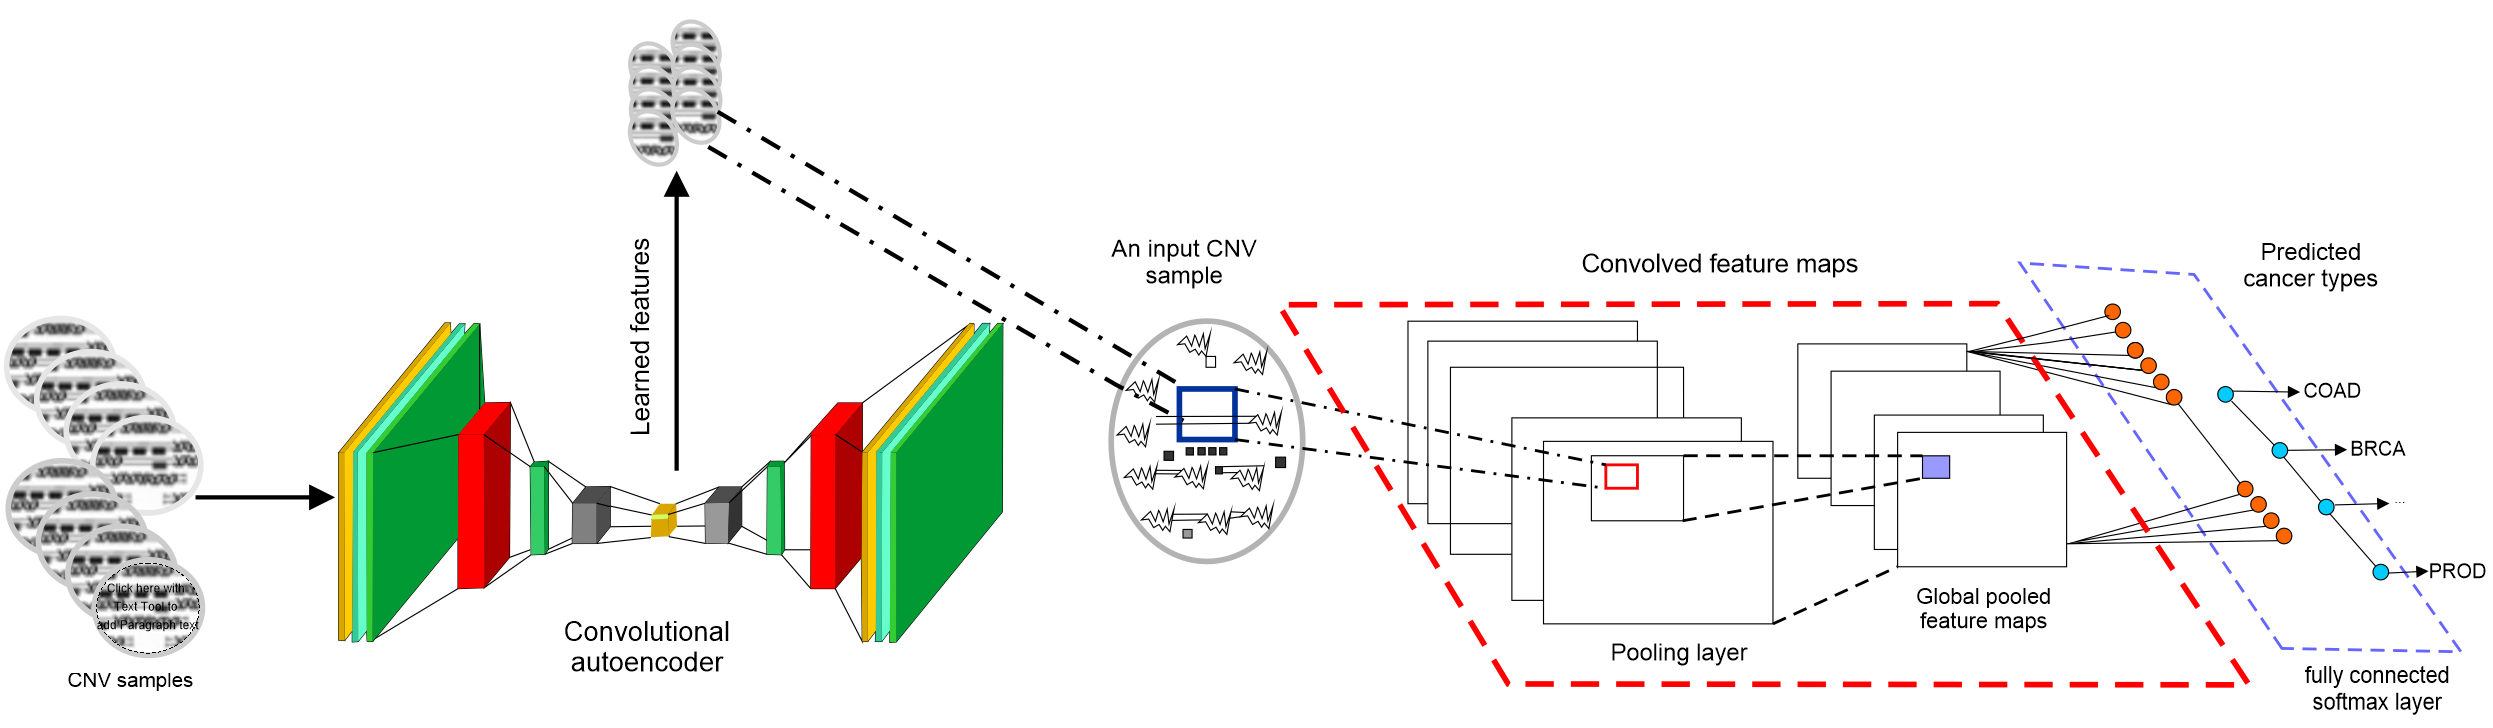
\includegraphics[width=0.9\textwidth,height=40mm]{images/cae2.png}	
    \caption{Schematic representation of the CAE classifier~\cite{karimACCA2019}}
	\label{fig:cae}
\end{figure*}

\hspace*{3.5mm} Especially, it is a major methodological guide for the correct tuning of the model capacity, progressively augmenting it to attain sparsity, or conversely reducing the dimension of the network removing links to zeroed out neurons~\cite{sparseAE}. As discussed in literature~\cite{karimBIB2019,karim2018recurrent}, due to the sparsity of $L_1$ regularization, sparse AEs actually learns better representations such that the activation are sparser, which makes it perform better than an original AE without $L_1$ regularization. By doing so an AE is actually learning latent representations instead of redundant information in our input data. 

%\subsubsection{CAE network construction}
\hspace*{3.5mm} Being motivated by several reasons, we constructed a CAE, which is architecturally a 19-layer autoencoder, in which a batch normalization layer is used after every conv layer and the ReLu activation function in every layer except for last layer that uses a Softmax activation function. From the given CNV samples, a convolutional layer in the encoder calculates the feature map. The pooling layer is calculated by down-sampling the convolutional layer by taking the maximum value in each non-overlapping sub-region. The CAE classifier contains of two parts: i) the CAE autoencoder and ii) the classifier. The CAE autoencoder part has the following structure: 

\begin{itemize}[noitemsep]
    \scriptsize
        \item Input layer: each CNVs sample is reshaped from 1 x 20,736 to 144 x 144
        \item Convolutional layer: of size 32 x 20,736 (i.e. 144 x 144) 
        \item Batch normalization layer: of size 32 x 20,736
        \item Convolutional layer: of size 32 x 20,736
        \item Batch normalization layer: of size 32 x 10,368
        \item Max-pooling layer: of size 32 x 10,368
        \item Convolutional layer: of size 64 x 10,368
        \item Batch normalization layer: of size 64 x 10,368
        \item Convolutional layer: of size 64 x 10,368
        \item Batch normalization layer: of size 64 x 10,368
        \item Convolutional layer: of size 128 x 10,368
        \item Batch normalization layer: of size 128 x 10,368
        \item Convolutional layer: of size 128 x 10,368
        \item Batch normalization layer: of size 128 x 10,368
        \item Convolutional layer: of size 128 x 10,368
        \item Batch normalization layer: of size 128 x 10,368
        \item Convolutional layer: of size 64 x 10,368
        \item Batch normalization layer: of size 64 x 10,368
        \item Upsampling layer: of size 64 x 20,736 
        \item Convolutional layer: of size 1 x 20,736.
\end{itemize}

\hspace*{3.5mm} After training the CAE, we remove the decoder components by making the first 19 layers trainable false\footnote{Since the encoder part is already trained}. On top of these components, we add a flattening layer, followed by a fully connected dense layer of size 128, followed by a Softmax output unit of 14, i.e., the number of classes. 

\subsection{Network training and neural ensemble} %all human genes
We train the networks in two steps: i) first, we train each network independently; and ii) we create multiple snapshots of both networks before applying MAE. While training the Conv-LSTM and CAE networks, network parameters were initialized with Xavier initialization~\cite{xavier} and trained using AdaGrad- a first-order gradient-based optimization technique to optimize the categorical cross-entropy loss \cref{eq:cce3} of the predicted cancer types vs actual cancer types. On the other hand, the Softmax activation function is used in the output layer for the probability distribution over the classes. The hyperparameters are defined in grid search and 10-fold cross-validation by varying learning rates and different batch sizes. Further, we observe the performance by adding the Gaussian noise layers followed by Conv and LSTM layers to improve model generalization and reduce overfitting. 

\vspace{-2mm}
\begin{equation} 
    E_{c} = \sum_{i, j, k} T_{i, j, k} \log P_{i, j, k}+\left(1-T_{i, j, k}\right) \log \left(1-P_{i, j, k}\right)
    \label{eq:cce3}
\end{equation} 

\begin{figure}
    \centering
    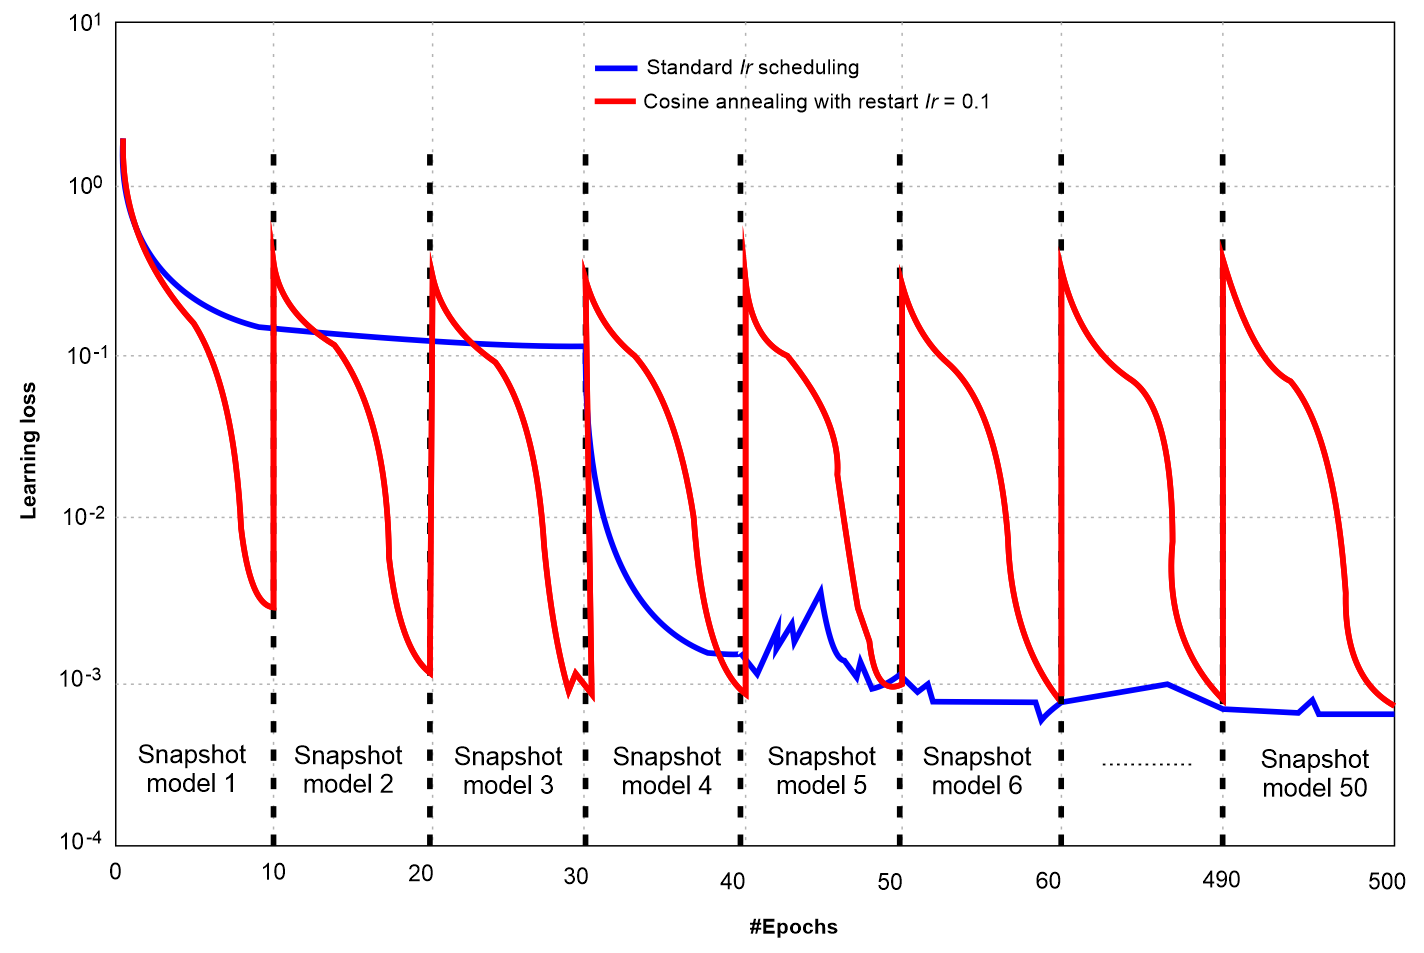
\includegraphics[width=0.75\textwidth,height=60mm]{images/ca.png}
    \caption{Training loss of Conv-LSTM network with standard learning rate~(blue) vs. cosine annealing~(red): intermediate models~(dotted lines) form an ensemble at the end of training~\cite{karimACCA2019}}
    \label{fig:ca}
    \vspace{-2mm}
\end{figure}

\hspace*{3.5mm} As discussed in \cref{chapter:preli}, model ensemble technique helps the neural network to achieve improved performance compared to the predictions from a single model by reducing the generalization error. We hypothesize\footnote{\textbf{$H_3$:} a neural ensemble method by combining several deep architectures already proven to be more effective than structures solely based on a single model~\cite{karimACCA2019}} that a neural ensemble method by combining several deep architectures can be more effective than structures solely based on a single model~\cite{karimACCA2019}. We achieved this using cyclic annealing cosine annealing~(CAC), which aggressively but systematically changes the learning rate~(LR) over epochs to produce different network weights~\cite{loshchilov2016sgdr}. We train multiple model snapshots during a single training run and combine their predictions to make an ensemble prediction called snapshot ensemble~\cite{huang2017snapshot}. 

\hspace*{3.5mm} The CAC requires total training epochs, maximum learning rate, and number of cycles, as well as the current epoch number making the initial LR and the total number of training epochs as two hyperparameters. Hence, CAC will have an effect of starting with a large LR, which is relatively rapidly decreased to a minimum value before being dramatically increased again to the following LR for the given epoch~\cite{huang2017snapshot}. CAC aggressively but systematically changes the learning rate over training epochs to produce very different network weights~\cite{loshchilov2016sgdr} as outlined in~\cref{fig:ca}. 

\begin{equation}
    \label{eq:lr-cosine}
    \alpha(t)=\frac{\alpha_{0}}{2}\left(\cos \left(\frac{\pi \bmod (t-1,\lceil T / M\rceil)}{\lceil T / M\rceil}\right)+1\right)
\end{equation}

\begin{figure}
    \centering
        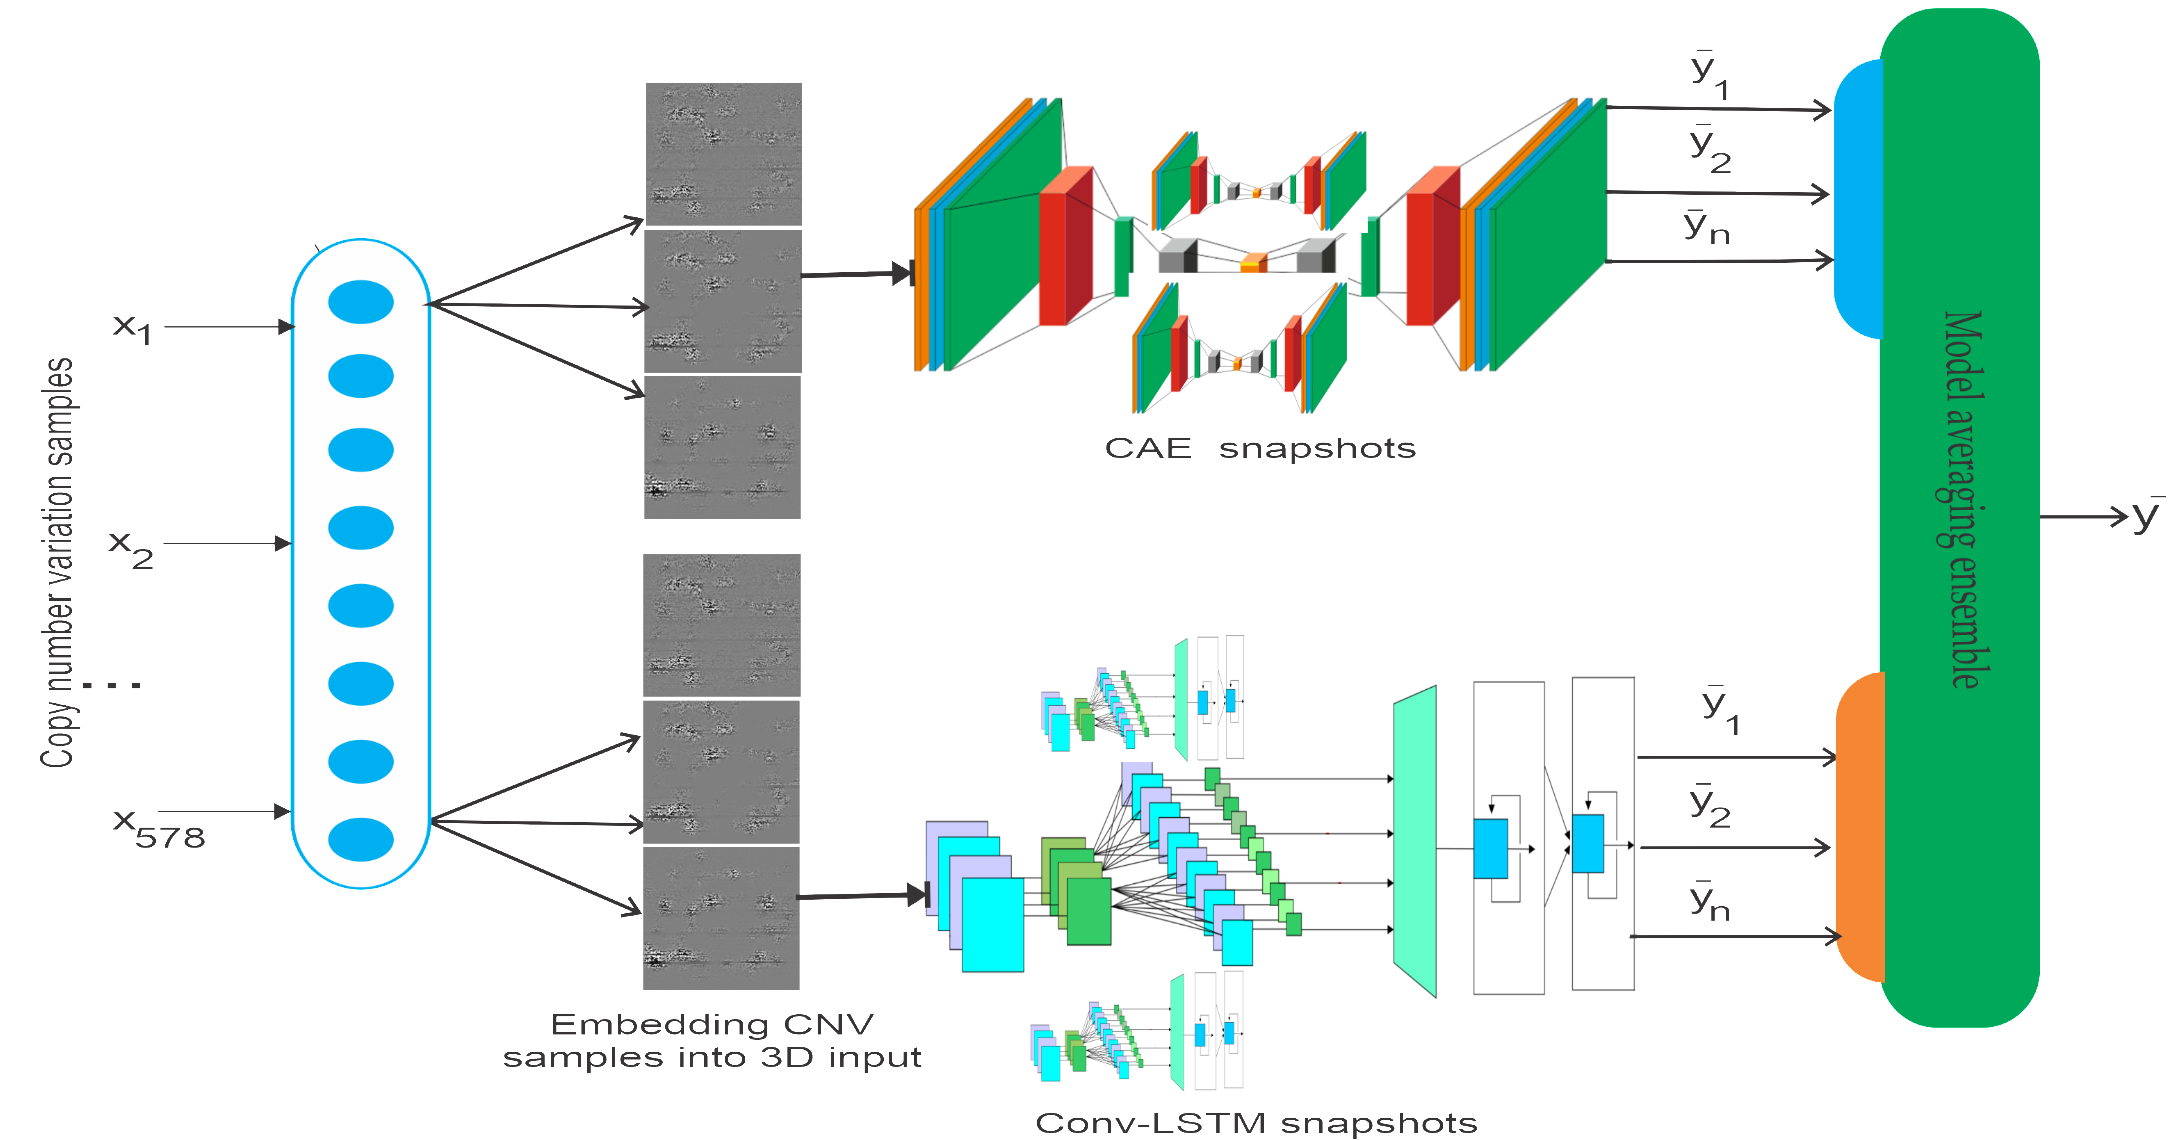
\includegraphics[width=0.8\textwidth,height=50mm]{images/mae_model_v2.png}
    \caption{Model averaging ensemble of Conv-LSTM and CAE snapshots~\cite{karimACCA2019}}
    \label{fig:mae}
    \vspace{-2mm}
\end{figure}

\hspace*{3.5mm} In \cref{eq:lr-cosine}, $\alpha(t)$ is the LR at epoch t, $\alpha_0$ is the maximum LR, $T$ is the total epoch, $M$ is the number of cycles, $mod$ is the modulo operation, and square brackets indicate floor operations. During the training of the ensemble model, we set total epochs, maximum learning rate, number of cycles, and the current epoch number, but we make the initial learning rate and the total number of epochs two hyperparameters as required. After training the network for $M$ cycles, best weights at the bottom of each cycle are saved as the snapshot of each model, which gives us $M$ model snapshots. The network undergoes several LR annealing cycles, converging to and escaping from multiple local minima during snapshot ensembling, followed by the ensemble prediction at test time is the average of the last $m$ model's Softmax outputs, where $m \leq M$. If $\mathbf{x}$ is a test sample, and $h_i \left(\mathbf{x} \right)$ is the softmax score of snapshot $i$, the final output is the simple mean of the last $m$ models shown in equation \ref{eq:mae}, giving the lowest test error~\cite{huang2017snapshot}. 

\vspace{-2mm}
\begin{equation}
    h_{\mathrm{MAE}}=\frac{1}{m} \sum_{0}^{m-1} h_{M-i}(\mathrm{x})
    \label{eq:mae}
\end{equation}

\hspace*{3.5mm} Finally, all the snapshots are collected and used in the final ensemble using MEA as shown in \cref{fig:mae}. Although, each model's weights are subjected to the dramatic changes during training for the subsequent LR cycle, CAC allows the learning algorithm to converge to a different solution. The final output is the simple mean of the last $m$ models in \cref{eq:mae}, giving the lowest test error as suggested in~\cite{huang2017snapshot}. 

%\subsection{Hyperparameter tuning}
%\label{ht}
\hspace*{3.5mm} We perform the hyperparameter optimization through a random search and 5-fold cross-validation tests. First, we optimize the parameters for the individual model, followed by the optimization of the ensemble model. While training the Conv-LSTM and CAE, in each of 5 runs, 70\% of the data is used for the training, 30\% for the evaluation, and 10\% from the training set is used for the validation of networks to optimize the learning rate, batch size, number of filters, kernel size, dropout probability, and Gaussian noise probability. For pretraining the CAE, 90\% of data is used for the training, and 10\% of the data is used for validation. When we train the ensemble model, we set number of epochs~(NE) to 500, maximum learning rate to 1.0, and number of cycles~(NC) to NE/10, giving 50 snapshots for each model for 50 cycles through a grid search, since an exhaustive optimization would be too computationally expensive. %Further, we only use a single object property to test how results change with each choice of parameter, due to computational constraints. 

\section{Experiments}\label{chapter_3:results}
We carried out several experiments based on protein-coding genes and oncogenes. By using each network and CNV representation, cancer type predictions were experimented separately. The results of each experiment with a comparative analysis will be discussed in detail in this section. 

\subsection{Experiment setup}
We report the results using macro-averaged precision and recall since classes are imbalanced. We did not report F1-scores since it is significant only when the value of precision and recall are very different. Further, for cancer diagnosis, it is important to have both high precision and recall. Hence, results with very different precision and recall are not useful in cancer diagnosing and tumor type identification. The MAE is then followed to report the final predictions. 

\subsection{Analysis of individual model}
Classification accuracies using oncogenes and all non-coding genes vary. In particular, using protein-coding genes, classifiers perform moderately well, giving accuracies of 72.96\% and 76.77\% with Conv-LSTM and CAE network, respectively. Since the classes are imbalanced, only the accuracy will give a very distorted estimation of the cancer types. Class-specific classification reports are thus shown in \cref{table:codingene} and \cref{table:resultoncogene}. 
As shown in~\cref{table:codingene}, precision and recall for majority cancer types were moderately high in which CAE performed mostly better than Conv-LSTM network. In particular, CAE classifier can classify COAD, GBM, KIRC, BRCA, LUSC, and PRAD more confidently~(at least 82.50\% of the cases). While, Conv-LSTM classified the OV tumor samples more accurately than CAE classifier~(83.56\% vs 76.13\%). The downside is that both classifiers have made a substantial amount of mistakes e.g., CAE can classify STAD and UCEC tumor cases only 65\% and 68\% accurately. Whereas, the Conv-LSTM network made more mistakes particularly for the STAD, BLCA, THCA, UCEC, LUAD, and LGG tumor samples. 

\begin{table} [h]
\caption{Performance on cancer type prediction using non-coding genes}
\label{table:codingene} %RF Confusion Matrix all genes Subtype
    \begin{center}
        \vspace{-5mm}
    \scriptsize
        \begin{tabular}{l|ll|ll|l}
        \hline
        \rowcolor{Gray}
        {} & \multicolumn{2}{c}{\textbf{Conv-LSTM~(72.96\%)}} & \multicolumn{2}{c}{\textbf{CAE~(76.77\%)}} &  {} \\\hline
        \textbf{Tumor type} & \textbf{Precision} &  \textbf{Recall}  & \textbf{Precision} &  \textbf{Recall} & \textbf{Support} \\\hline
        COAD    & 0.6981  &  0.7325 & 0.7924 &    0.8250 & 133  \\\hline
        GBM     & 0.8127  &  0.8275 & 0.8247 &   0.8765  & 151  \\\hline
        KIRC    & 0.8013  &  0.7335 & 0.8331 &   0.8468  & 150  \\\hline
        LGG     & 0.8250  &  0.6935 & 0.8642 &   0.7835 & 120  \\\hline
        LUAD    & 0.6835  &  0.6584 & 0.6992 &   0.7238 & 136  \\\hline
        LUSC    & 0.6937  &  0.7294 & 0.7438 &   0.8352 & 132  \\\hline
        OV      & 0.7539  &  0.8356 & 0.8365 &   0.7613 & 145  \\\hline
        UCEC    & 0.6645  &  0.6829 & 0.7435 &   0.6834 & 131  \\\hline
        BRCA    & 0.7357  &  0.7587 & 0.7954 &   0.8386 & 269  \\\hline
        HNSC    & 0.7134  &  0.7235 & 0.6853 &   0.7542 & 141  \\\hline
        THCA    & 0.6967 &  0.6959 & 0.7025 &   0.7654 & 121  \\\hline
        PRAD    & 0.7225  &  0.7934 & 0.8395 &   0.8345 & 124  \\\hline
        STAD    & 0.6528  &  0.6917 & 0.6776 &   0.6512 & 113  \\\hline
        BLCA    & 0.7356  &  0.6589 & 0.7925 &   0.7489 & 108  \\\hline
        \rowcolor{LightCyan}
        \textbf{Avg/total} & \textbf{0.7278} &    \textbf{0.7296} & \textbf{0.7593} &    \textbf{0.7677} & \textbf{1974}  \\\hline
        \end{tabular}
        \vspace{-4mm}
    \end{center}
\end{table}

\hspace*{3.5mm} On the other hand, although the tumor-specific classification accuracies varied across classes, the overall accuracies increased moderately and reached 74.25\% and 78.32\% using Conv-LSTM and CAE, respectively. As seen in~\cref{table:resultoncogene}, the precision and recall for most of the cancer types are than that of protein-coding gene-based CNVs. Similar to the previous experiment, CAE performed mostly better than the Conv-LSTM network across tumor types. In particular, the CAE classifier can correctly classify COAD, GBM, OV, UCEC, PRAD, and BLCA in at least 80\% of the cases showing higher confidence. 

\begin{figure}[h]
	\centering
	\begin{subfigure}{0.48\linewidth}
		\centering
		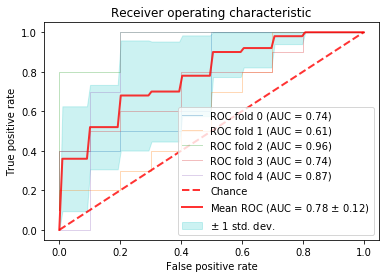
\includegraphics[width=\linewidth]{images/download1.png}
		\caption{Using CAE classifier}
	\end{subfigure}
	\begin{subfigure}{0.48\linewidth}
		\centering
		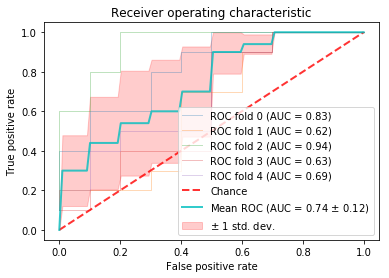
\includegraphics[width=\linewidth]{images/download2.png}
		\caption{Using Conv-LSTM network}
	\end{subfigure}
	\caption{The ROC curves for Conv-LSTM and CAE models across folds} 
	\label{fig:roc}
	 \vspace{-2mm}
\end{figure}

\begin{table}[h]
\caption{Performance on cancer type prediction using oncogenes }
\label{table:resultoncogene} 
\begin{center}
    \scriptsize
    \vspace{-5mm}
    \begin{tabular}{l|ll|ll|l}
        \hline
        \rowcolor{Gray}
        {} & \multicolumn{2}{c}{\textbf{Conv-LSTM (74.67\%)}} & \multicolumn{2}{c}{\textbf{CAE (78.32\%)}} &  {} \\\hline
        \textbf{Tumor type }& \textbf{Precision} &  \textbf{Recall}  & \textbf{Precision} &  \textbf{Recall} & \textbf{Support~(CAE)} \\\hline
        COAD   & 0.7785 & 0.7564 & 0.8265 & 0.8193 & 133  \\\hline
        GBM    & 0.8254 & 0.8330 & 0.8433 & 0.8524 & 151  \\\hline
        KIRC   & 0.7753 & 0.7835 & 0.8172 & 0.8035 & 150  \\\hline
        LGG    & 0.8235 & 0.7136 & 0.7976 & 0.8031 & 120  \\\hline
        LUAD   & 0.7520 & 0.7351 & 0.7584 & 0.7674 & 136  \\\hline
        LUSC   & 0.7528 & 0.6475 & 0.7139 & 0.7256 & 132  \\\hline
        OV     & 0.8327 & 0.8407 & 0.8665 & 0.8538 & 145  \\\hline
        UCEC   & 0.7726 & 0.7625 & 0.8732 & 0.8412 & 131  \\\hline
        BRCA   & 0.7956 & 0.8075 & 0.8012 & 0.7965 & 269  \\\hline
        HNSC   & 0.8253 & 0.6932 & 0.7025 & 0.6929 & 141  \\\hline
        THCA   & 0.7953 & 0.8025 & 0.7429 & 0.7581 & 121  \\\hline
        PRAD   & 0.8267 & 0.8237 & 0.8781 & 0.8626 & 124  \\\hline
        STAD   & 0.7924 & 0.6945 & 0.7632 & 0.7737 & 113  \\\hline
        BLCA   & 0.8368 & 0.7979 & 0.8623 & 0.8553 & 108  \\\hline
        \rowcolor{LightCyan}
        \textbf{Avg/total} &   \textbf{0.7543}    &  \textbf{0.7467} &    \textbf{0.7945}   &  \textbf{0.7832} & \textbf{1974} \\\hline
    \end{tabular}
     \vspace{-6mm}
    \end{center}
\end{table}

\hspace*{3.5mm} On the contrary, Conv-LSTM classified the BRCA and THCA tumor samples more accurately than the CAE classifier. The downside is that both classifiers have made substantial mistakes, too. For example, CAE could classify HNSC and LUSC tumor samples accurately in only 69\% and 72\% of the cases. Whereas, the Conv-LSTM network made more mistakes, particularly for the STAD, HNSC, LUSC, and LGG tumor samples. In summary, both classifiers performed moderately well except for certain types of tumor cases such as STAD, HNSC, BLCA, THCA, UCEC, LUAD, LUSC, and LGG. The ROC curves in \cref{fig:roc} based on CNVs from oncogene shows that AUC scores generated by both the \texttt{Conv-LSTM} model and \texttt{CAE} classifier are consistent across folds, and AUC scores generated by the \texttt{CAE} classifier are about 4\% better than that of the \texttt{Conv-LSTM} network.

\begin{figure}[h]
	\centering
	\begin{subfigure}{0.48\linewidth}
		\centering
		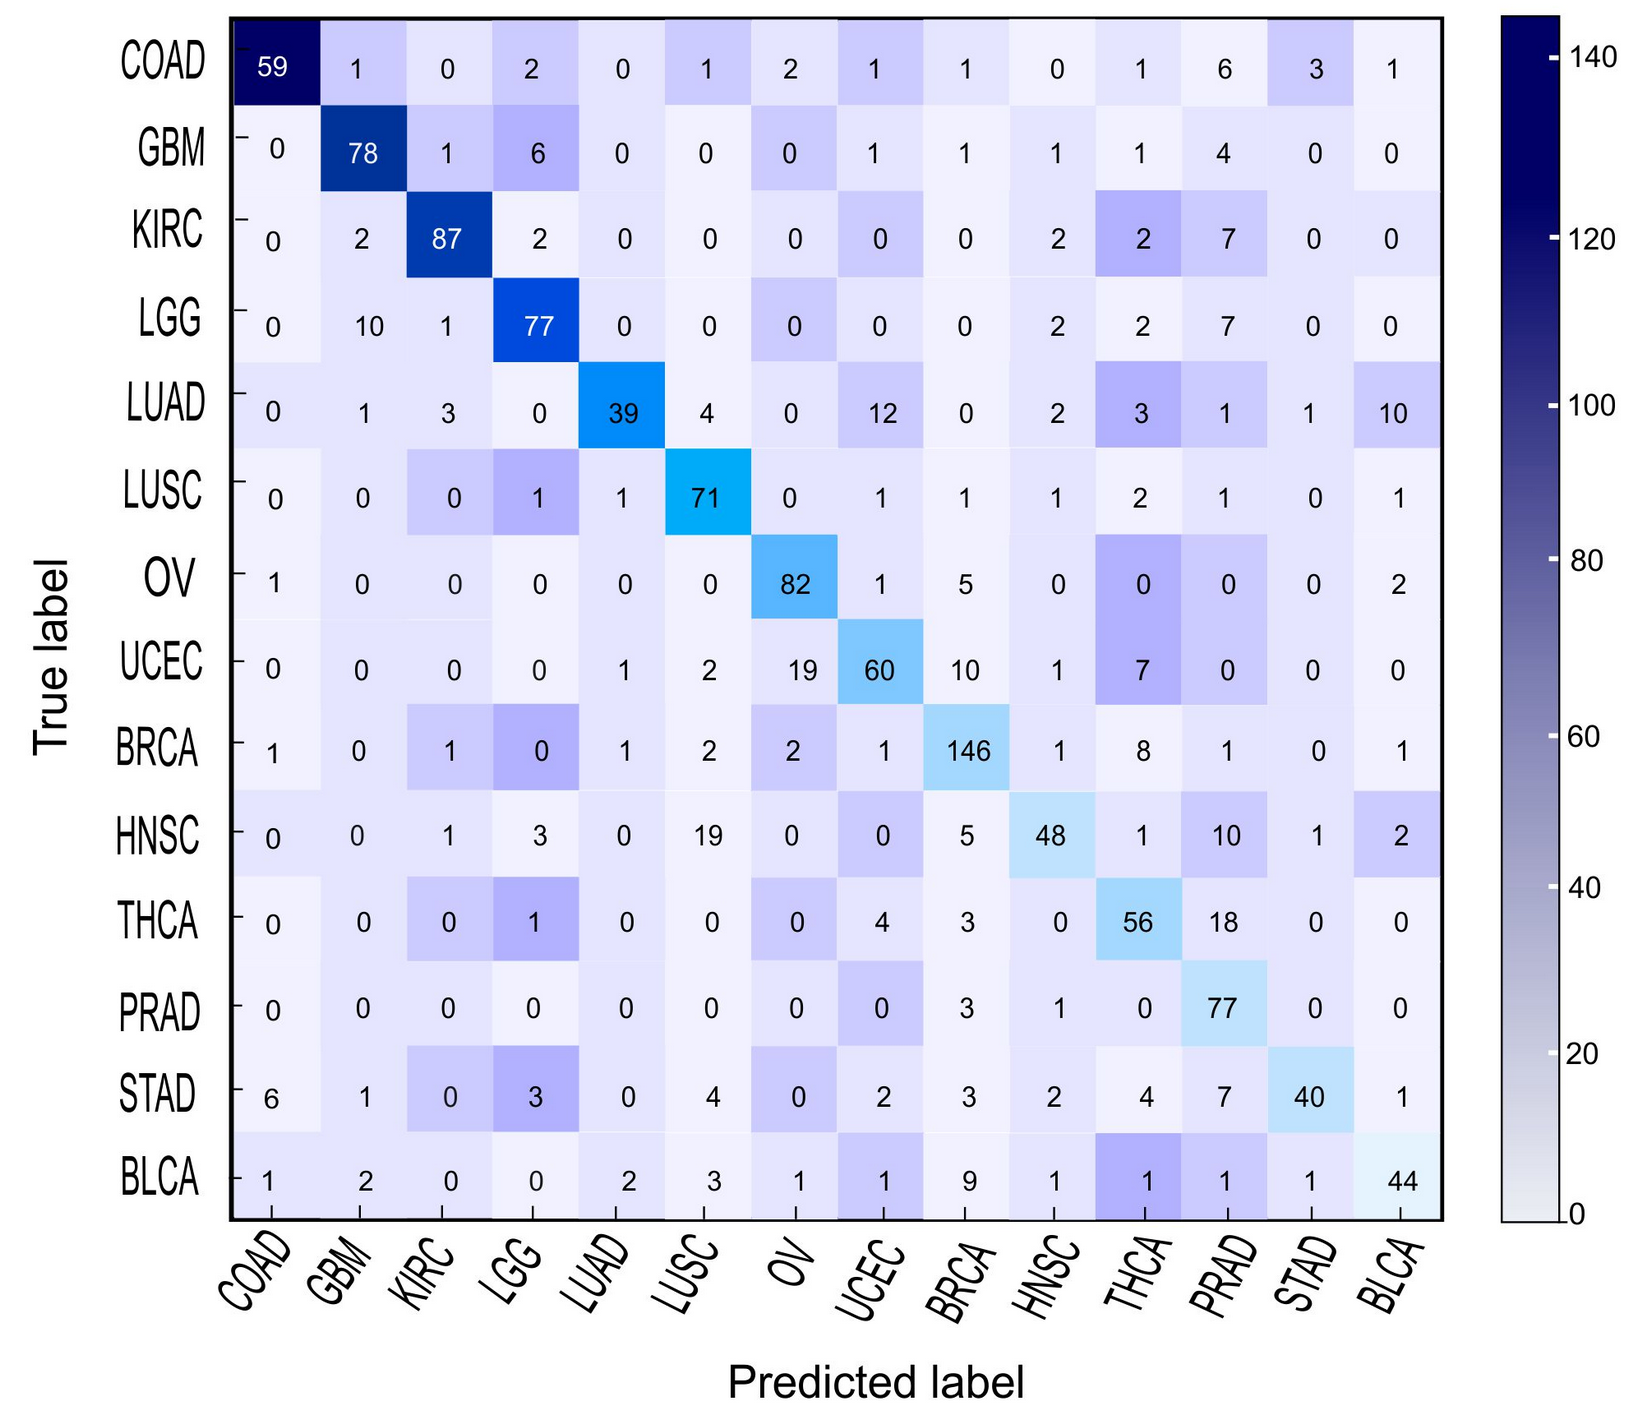
\includegraphics[width=0.95\linewidth]{images/cm1.png}
		\caption{Using coding genes based CNVs}
        \label{fig:cm_1}
	\end{subfigure}
	\begin{subfigure}{0.48\linewidth}
		\centering
		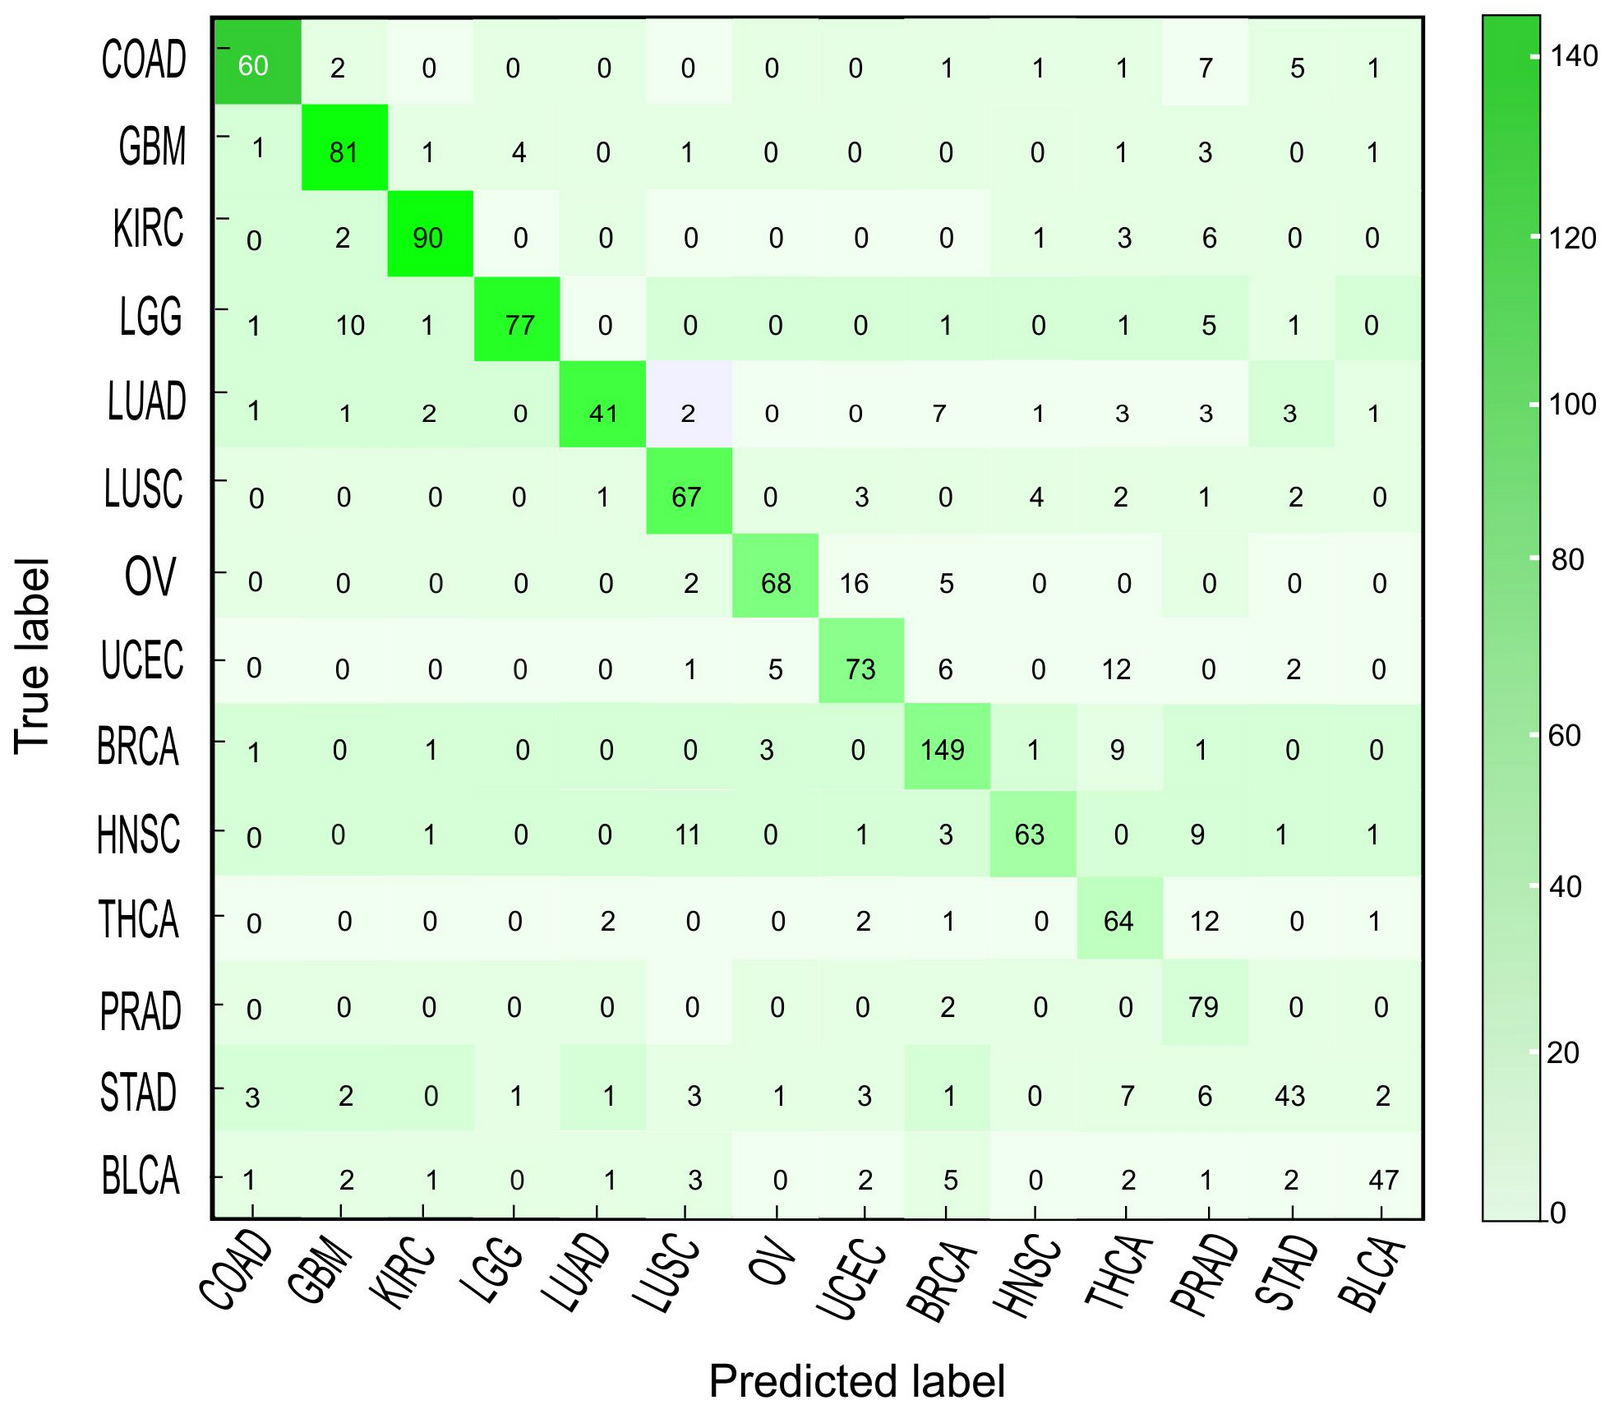
\includegraphics[width=0.95\linewidth]{images/cm2.png}
		\caption{Using oncogenes based CNVs}
        \label{fig:cm_2}
	\end{subfigure}
	\caption{Confusion matrices of the ensemble classifier} 
	\label{fig:cms}
	 \vspace{-4mm}
\end{figure}

\subsection{Analysis of the ensemble model}
The ensemble classifier shows about 2\% and 4\% performance boost across classes and overall in the cases of oncogenes and protein-coding gene-based experiment, respectively. The accuracy looks easy enough but makes no distinction between classes e.g., when a doctor makes a medical diagnosis that a patient has cancer, but in reality, the patient does not~(i.e., false positive). This has very different consequences than making the call that a patient does not have cancer when he actually does~(i.e., false negative). A more detailed breakdown of correct and incorrect classifications for each class using the confusion matrices is shown in \cref{fig:cms}, which correspond to ground truth labels vs. the predictions made.

\hspace*{3.5mm} As shown, there are significant accuracy improvements in case of STAD, HNSC, BLCA, THCA, UCEC, and LUSC tumor types. In case of UCEC and LUSC cancer types, not only are the accuracies increased slightly, but also the false positive rates are reduced significantly. On the contrary, using oncogenes, the classifiers were less confused among tumor types, except for the LGG, HNSC, and THCA tumor types. Despite these improvements, there is still high confusion among LUAD, HNSC, and LGG, which is because features from these tumor samples are highly correlated. We could not find an exact reason for such behavior. Perhaps, a more gene-specific CNV analysis is required to confirm such correlations. However, poor and imbalance training might be one of the reasons. 

%\section{Discussion}\label{chapter_3:discussion}
\hspace*{3.5mm} Some previous studies focused on using CNVs datasets~\cite{zhang2016classification,elsadek2018supervised} from cBioPortal for Cancer Genomics. They applied incremental feature selection methods before training classic ML models and managed to achieve classification accuracy of 75\% and 85\%~(by Zhang et al. and Sanaa F. et al., respectively). Since we have more samples from different source to train DL algorithms, a one-to-one comparison was not viable. Our proposed approach achieved 80\% classification accuracy, which is about 6\% better than our previous approach~\cite{karim2018a2ic} w.r.t. every metric. Considering an accuracy of 80\% for cancer type prediction, we cannot claim that our model’s confidence is very high. This is for several reasons, such as lack of training samples, poor training, and data sparsity. The latter reason caused each network to produce high training and validation loss of error optimization during the training phase, giving lower accuracy. 

\hspace*{3.5mm} Data sparsity evolved because, on average, only 422 samples per tumor were used for the training. This is fairly low for such high-dimensional complex data. As a result, models were not trained well enough to identify subtle differences among tumors types. We lacked enough training samples compared to the complex dataset, as deep architectures usually expect more samples to get trained well. %For the same reason, there was a lack of samples to perform model validation during 5-fold cross-validation. 
Another reason for poor training might be an imbalanced dataset. As we can see, some cancer types, such as BRCA, has 2.5 times more training samples than other tumors. For example, STAD and BLCA have at least 15\% sample difference with other tumor types. These two tumors have very low classification accuracy, where about half of the samples were misclassified. Another unavoidable issue is that sometimes experiments with different types of ML algorithms show different results. Depending on the genome sequencing and several algorithms for CNV calling,  tools might produce different copy numbers with different CNV lengths and segmentation means, which may change the results drastically.

\section{Chapter Summary} \label{chapter_3:conclusion}
In this chapter, we developed a snapshot neural ensemble method for cancer-type prediction based on CNVs data using two deep architectures called \texttt{Conv-LSTM} and \texttt{CAE}. Our ensemble method is based on cosine annealing techniques, which create multiple model snapshots of these networks, followed by MAE technique to combine the predictive power of these architectures. Experimental results show that CNVs are not only useful for predicting certain types of cancer but also show an obvious association with cancer growth. Another type of data~(e.g., DNA methylation, gene expression, somatic mutations) can be used to create prediction model in a similar fashion of single modality-based cancer typing we discussed in this chapter. The downside of this single modality-based cancer typing method is that the findings are not validated with other annotations or scientific literature, which is why it cannot confirm if the identified genes are biologically relevant. Therefore, it is literally a `black-box' model. 

\hspace*{3.5mm} Further, since multiple factors are involved in cancer diagnosis (e.g., estrogen receptor~(ER), progesterone receptor~(PGR), and human epidermal growth factor receptor 2~(HER2/neu) statuses for breast cancer), providing AI-based diagnoses might not be accurate solely based on CNVs. We require multimodal features based on DNA methylation, GE, miRNA expression, and CNVs data by creating a multiplatform network to support each data type. Lastly, a DL approach using CNV data along with other types of genomics data from different cohorts such as DNA methylation, GE, and mutations will be more reliable. In the next chapter, we extend this work increasing the number of samples for training, testing, and validation, by combining samples from PanCancerAtlas. We employ a multimodal neural network architecture to combine features interpret the combinations to predict the cancer subtypes. 
